% Build from this folder with: latexmk -pdf pathwise_loss_presentation.tex
\documentclass[aspectratio=169,9pt]{beamer}

\graphicspath{{theme-assets/}}
\usetheme{oxfordmaths}

\usepackage{amsmath,amssymb,booktabs,array,graphicx,mathtools}
\usepackage{tikz}
\usetikzlibrary{positioning,arrows.meta}

\definecolor{softblue}{RGB}{232,239,247}
\definecolor{softorange}{RGB}{252,239,229}
\definecolor{softgrey}{RGB}{245,246,248}
\definecolor{darkgrey}{RGB}{70,76,84}

\setbeamerfont{title}{size=\LARGE,series=\bfseries}
\setbeamerfont{frametitle}{size=\Large,series=\bfseries}
\setbeamerfont{block title}{series=\bfseries}
\setbeamercolor{block title}{fg=white,bg=oxfordblue}
\setbeamercolor{block body}{fg=black,bg=softblue}
\setbeamercolor{alertblock title}{fg=white,bg=oxfordblue}
\setbeamercolor{alertblock body}{fg=black,bg=softblue}
\setbeamertemplate{itemize item}{\color{oxfordblue}$\blacktriangleright$}
\setbeamertemplate{itemize subitem}{\color{oxfordblue}$\bullet$}

% One paragraph gap and one table row height for the whole deck. Frames carry no
% manual \vspace, so spacing cannot drift between slides.
\setlength{\parskip}{0.55em}
\renewcommand{\arraystretch}{1.35}
\setbeamertemplate{blocks}[rounded][shadow=false]

\newcommand{\Jtwo}{J_2}
\newcommand{\result}[1]{\textcolor{oxfordblue}{\bfseries #1}}
\newcommand{\caveat}[1]{\textcolor{oxfordblue}{\bfseries #1}}
\newcommand{\metricbox}[2]{%
  \begin{beamercolorbox}[rounded=true,sep=0.7em,wd=\linewidth]{#1}
    #2
  \end{beamercolorbox}}

\title[Pathwise losses]{Principled loss functions\\
for continuous-time learning}
\author{Haoping Qiu}
\institute{Mathematical Institute, University of Oxford\\DataSig}
\date[September 2026]{3 August to 10 September 2026}

%% Section divider: empty frame title so header rule and logos stay, and
%% frame counts in the footer.
\newcommand{\dividerframe}[1]{%
  \begin{frame}{\strut}%
    \vfill
    \centering
    {\usebeamercolor[fg]{frametitle}\huge\bfseries #1}\par
    \vfill
  \end{frame}%
}

\begin{document}

\begin{frame}[plain]
  \titlepage
\end{frame}

\dividerframe{Motivation}

\begin{frame}{Motivation}
Observed time series are finite sequences of time-stamped values. Sequence to sequence models are trained using pointwise losses such as mean squared error (MSE).

Continuous time models such as neural differential equations enable path-to-path learning, where inputs and outputs are continuous-time trajectories.

An open question is which loss functions are best suited to path-to-path learning, as previous work has shown that pointwise objectives can overfit local noise and fail to capture temporal structure (Ramsay and Silverman, 2005; Kudrat et al., 2025).
\end{frame}

\begin{frame}{Pointwise agreement and path error}
  \small
  \textbf{Project question}\par
  The project studies definitions of path closeness and how each definition changes the learned path or operator. Let $0=t_0<\cdots<t_m=T$ be observation times and suppose two continuous predictions satisfy
  \[
    \widehat Y_A(t_j)=\widehat Y_B(t_j)=Y(t_j),
    \qquad j=0,\ldots,m.
  \]
  Both have zero pointwise mean squared error,
  \[
    \operatorname{MSE}(\widehat Y_\ell,Y)
    :=\frac1{m+1}\sum_{j=0}^{m}\|\widehat Y_\ell(t_j)-Y(t_j)\|_2^2=0,
    \qquad \ell\in\{A,B\},
  \]
  yet their behaviour between observations can differ. Their elapsed-time errors may therefore differ:
  \[
    \Jtwo(\widehat Y_A,Y)
    \quad\text{need not equal}\quad
    \Jtwo(\widehat Y_B,Y),
    \qquad
    \Jtwo(\widehat Y,Y):=\int_0^T\|\widehat Y(t)-Y(t)\|_2^2\,dt.
  \]

  \textbf{Role of discretisation}\par
  Although paths are stored at finitely many times, the loss still determines how the underlying paths are compared. Weighting, interpolation and feature representation each affect that comparison.

\end{frame}

\begin{frame}{Path-to-path learning}
  Functional-data analysis treats an input $X$ and target $Y$ as whole paths (Ramsay and Silverman, 2005):
  \[
    X\in\mathcal X:=C([0,T];\mathbb R^{d_x}),
    \qquad
    Y\in\mathcal Y:=C([0,T];\mathbb R^{d_y}).
  \]
  A parameterized model is an operator from input paths to predicted output paths:
  \[
    \mathcal F_\theta:\mathcal X\to\mathcal Y,
    \qquad
    \widehat Y_\theta:=\mathcal F_\theta(X),
    \qquad \theta\in\Theta.
  \]
  Given paired training paths $(X^{(i)},Y^{(i)})_{i=1}^{N}$ and a path loss $\mathcal L:\mathcal Y\times\mathcal Y\to[0,\infty)$, training selects
  \[
    \widehat\theta\in\underset{\theta\in\Theta}{\arg\min}
    \frac1N\sum_{i=1}^{N}
    \mathcal L\!\left(\mathcal F_\theta(X^{(i)}),Y^{(i)}\right).
  \]

  The loss $\mathcal L$ determines which discrepancies between predicted and target paths training treats as important.
\end{frame}

\begin{frame}{Loss functions}
  \small
  \begin{tabular}{>{\bfseries}p{0.18\textwidth}p{0.34\textwidth}p{0.385\textwidth}}
    \toprule
    Loss & Definition & Emphasis \\
    \midrule
    Pointwise MSE & $\displaystyle \frac1{m+1}\sum_{j=0}^{m}\|\widehat Y(t_j)-Y(t_j)\|_2^2$ & Each recorded point has equal weight \\
    Elapsed-time $\Jtwo$ & $\displaystyle \Jtwo(\widehat Y,Y):=\int_0^T\|\widehat Y(t)-Y(t)\|_2^2\,dt$ & Error accumulated over time \\
    Sobolev $H^1$ & $\displaystyle \Jtwo(\widehat Y,Y)+\kappa\int_0^T\|\dot{\widehat Y}(t)-\dot Y(t)\|_2^2\,dt$ & Values and local velocity for smooth paths \\
    Signature loss & $\displaystyle \|\Phi_M(\widehat Y)-\Phi_M(Y)\|_2^2$ & Ordered increments and interactions through depth $M$ \\
    \bottomrule
  \end{tabular}

  \vfill
  \textbf{Comparison principle}\par
  For the $H^1$ loss, $Y,\widehat Y\in H^1([0,T];\mathbb R^{d_y})$, dots denote weak time derivatives, and $\kappa>0$ balances value and derivative error (Ramsay and Silverman, 2005). Map $\Phi_M$ collects signature coordinates through level $M$ (Chen, 1957; Lyons et al., 2007). Each fitted path is evaluated under every metric.
\end{frame}

\begin{frame}{Integral norms and temporal order}
  Following the standard $L^p$ definition (Lieb and Loss, 2001), for residual path $e(t):=\widehat Y(t)-Y(t)$ and $1\leq p<\infty$ set
  \[
    \|e\|_{L^p}:=
    \left(\int_0^T\|e(t)\|_2^p\,dt\right)^{1/p}.
  \]
  If $\tau:[0,T]\to[0,T]$ preserves elapsed time, then
  \[
    \|e\circ\tau\|_{L^p}=\|e\|_{L^p}.
  \]
  Integral norms therefore record the size and duration of an error, but not the order in which its values occur.

  \vfill
  \begin{columns}[T,onlytextwidth]
    \begin{column}{0.47\textwidth}
      \textbf{Consequence for rough streams}\par
      A second-level perturbation can leave every coordinate value unchanged. Coordinate losses then respond by exactly zero, whatever their exponent or weighting.
    \end{column}
    \begin{column}{0.47\textwidth}
      \textbf{Contribution of signatures}\par
      Level $k$ is an iterated integral over $t_1<\cdots<t_k$, so it is built from ordering rather than from magnitude at aligned times.
    \end{column}
  \end{columns}
\end{frame}

\begin{frame}{Path signatures}
  Let $a<b$, let $Y:[a,b]\to\mathbb R^d$ have bounded variation, and let $M\in\mathbb N$. For $k=1,\ldots,M$, its signature levels and depth-$M$ truncation are
  \[
    S^{(0)}(Y)_{a,b}:=1,
    \qquad
    S^{(k)}(Y)_{a,b}
    :=\int_{a<t_1<\cdots<t_k<b}
      dY_{t_1}\otimes\cdots\otimes dY_{t_k},
  \]
  \[
    S^{\le M}(Y)_{a,b}:=
    \bigl(S^{(0)}(Y)_{a,b},\ldots,S^{(M)}(Y)_{a,b}\bigr),
  \]
  where $\otimes$ is the tensor product (Chen, 1957; Lyons et al., 2007). A machine-learning introduction appears in Chevyrev and Kormilitzin (2016).
  \begin{itemize}
    \item Level 1 records net displacement.
    \item Level 2 records ordered pair interactions. Its antisymmetric part records signed area.
    \item Higher levels record increasingly detailed ordered interactions.
  \end{itemize}
  \textbf{Truncation and localization}\par
  A global comparison uses one truncated signature over the full interval. A local comparison uses signatures over a partition, thereby retaining coarse information about where an ordered feature occurs.
\end{frame}

\dividerframe{Experiment A: fixed path}

\begin{frame}{Experiment A: target path}
  For $t\in[0,1]$, define
  \[
    a(t):=0.3\exp\!\left[-100\left(t-\tfrac14\right)^2\right],
    \qquad
    Y^\star(t):=
    \begin{pmatrix}
      \cos(2\pi t)+a(t)\cos(12\pi t)\\
      \sin(2\pi t)+a(t)\sin(12\pi t)
    \end{pmatrix}.
  \]
  The circular component gives the broad shape. The localized envelope $a(t)$ creates a short oscillatory burst near $t=0.25$.

  \begin{center}
    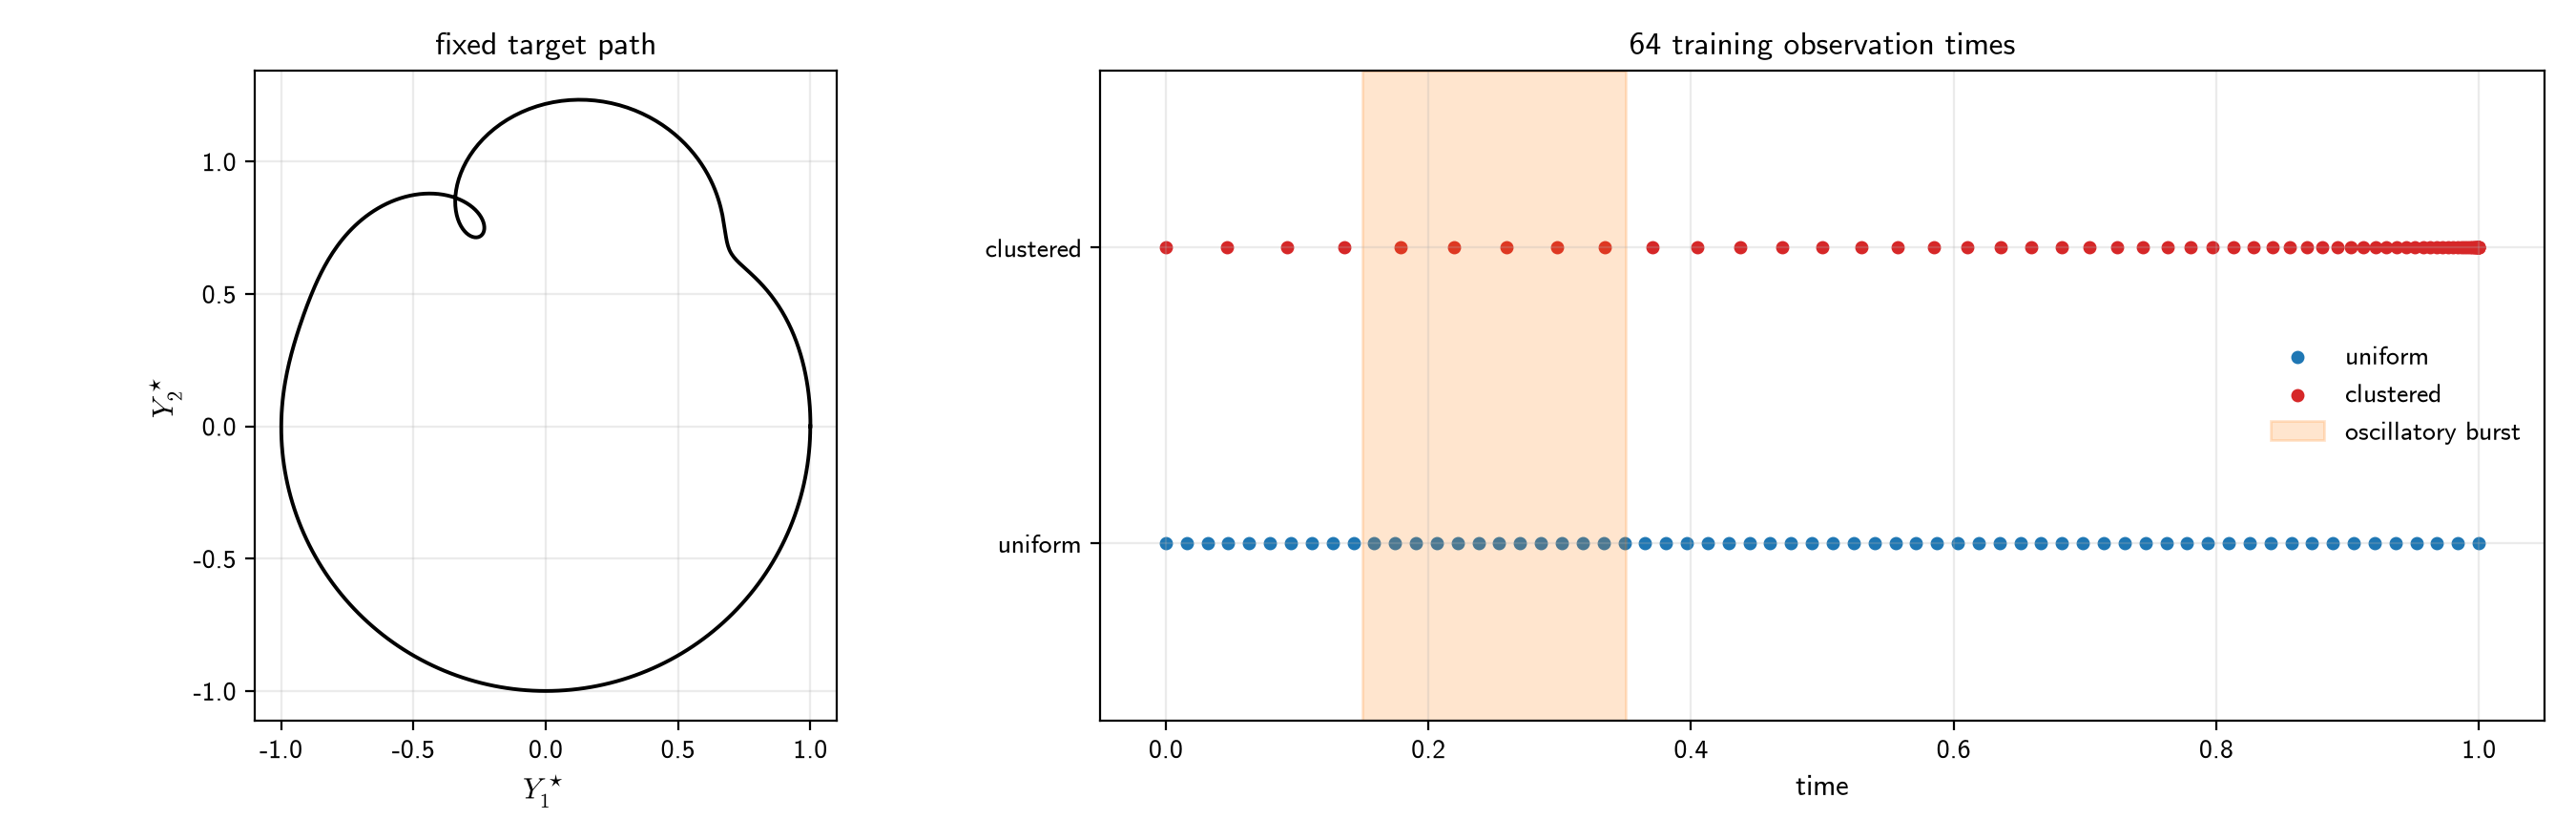
\includegraphics[width=0.92\linewidth]{assets/target_design.png}
  \end{center}
\end{frame}

\begin{frame}{Experiment A: model and comparison}
  A Neural ODE generates a continuous fitted path (Chen et al., 2018):
  \[
    z_\theta(0)=z_{0,\theta},
    \qquad
    \dot z_\theta(t)=f_\theta\!\left(t,z_\theta(t)\right),
    \qquad
    \widehat Y_\theta(t)=g_\theta\!\left(z_\theta(t)\right).
  \]
  Here $z_\theta(t)$ is the learned hidden trajectory, $f_\theta$ is a neural vector field, and $g_\theta$ maps the hidden state to two output coordinates. The restricted model has hidden dimension 2 and width 16. The expressive model has hidden dimension 8 and width 64.

  For each loss, the model fits the same target $Y^\star$ from 64 observations. The observation times are either uniform or clustered, while the initialization, optimizer and training budget remain matched. Evaluation compares every fitted path on the same dense grid under every metric.

  The experiment isolates how the training loss changes the path recovered from the same data and model family.
\end{frame}

\begin{frame}{Experiment A: loss comparisons}
  \begin{tabular}{>{\bfseries}p{0.23\textwidth}p{0.66\textwidth}}
    \toprule
    Comparison & Main idea \\
    \midrule
    MSE and $\Jtwo$ & Effect of elapsed-time weighting under clustered observations \\
    $H^1$ & Recovery of the short burst through direct velocity supervision \\
    Global signature & Structural agreement from one summary of the whole path \\
    Local signatures & Recovery of local structure when the partition is refined from 10 to 100 intervals \\
    \bottomrule
  \end{tabular}

  \vfill
  Every comparison uses matched initialization and optimization. Each fitted path is then evaluated under all losses on the same dense time grid, so a training objective is not judged only by its own score.
\end{frame}

\begin{frame}{Experiment A: anchored signature loss}
  For a two-dimensional output path $Y$, define the time-augmented path
  \[
    Z_Y(t):=(t,Y(t))\in\mathbb R^{d_Z},
    \qquad d_Z=3.
  \]
  The time channel makes the timing of motion visible to the signature. For an interval $I=[a,b]$, write
  \[
    \Delta S_I^{(k)}
    :=S^{(k)}(Z_{\widehat Y})_{a,b}-S^{(k)}(Z_Y)_{a,b}.
  \]

  \textbf{Anchor}\par
  Signatures do not change when a constant vector is added to every point of a path (Chen, 1957; Lyons et al., 2007). The additional term
  \[
    A_0(\widehat Y,Y):=\frac12\|\widehat Y(0)-Y(0)\|_2^2
  \]
  restores sensitivity to the starting position. Experiment A treats paths with different initial positions as different, so this information must be retained.

  \textbf{Level weights}\par
  Level $k$ has $d_Z^k$ tensor coordinates. Weight $d_Z^{-k}$ converts its squared Euclidean discrepancy into a mean squared discrepancy per coordinate, preventing dimension alone from favouring higher levels.
\end{frame}

\begin{frame}{Experiment A: global and local signature losses}
  The global objective compares one depth-four signature over the full path:
  \[
    \mathcal L_{\mathrm{global}}(\widehat Y,Y)
    :=A_0(\widehat Y,Y)
      +\sum_{k=1}^{4}d_Z^{-k}\|\Delta S_{[0,1]}^{(k)}\|_2^2.
  \]
  It measures overall ordered structure, but does not identify where within the interval a discrepancy occurs.

  Partition $[0,1]$ into $K$ intervals $I_b=[(b-1)/K,b/K]$. The local objective is
  \[
    \mathcal L_{\mathrm{local},K}(\widehat Y,Y)
    :=A_0(\widehat Y,Y)
      +\frac1K\sum_{b=1}^{K}\sum_{k=1}^{2}
        d_Z^{-k}\|\Delta S_{I_b}^{(k)}\|_2^2.
  \]
  Experiment A first uses $K=10$. Comparing signatures block by block retains coarse temporal location while keeping the representation small.
\end{frame}

\begin{frame}{Experiment A: depth and localization}
  For the three-dimensional time-augmented path, one depth-four signature contains
  \[
    3+3^2+3^3+3^4=120
  \]
  nonconstant coordinates. A depth-two signature contains $3+3^2=12$ coordinates, so ten local blocks also contain
  \[
    10(3+3^2)=120
  \]
  coordinates in total.

  The initial comparison therefore changes the structure of the representation while holding its raw size fixed:
  \begin{itemize}
    \item global depth four retains higher-order interactions but loses their location;
    \item local depth two discards levels three and four but retains coarse location.
  \end{itemize}
  In the local objective, factor $1/K$ averages rather than sums block discrepancies, so adding blocks does not increase the loss merely by adding terms.
\end{frame}

\begin{frame}{Experiment A: refined local signature loss}
  On an interval of length $h$, a level-$k$ signature scales approximately as $h^k$. Its squared discrepancy therefore scales as $h^{2k}$. Refining from a reference partition $K_0=10$ to $K=100$ would otherwise make the signature terms much smaller.

  The refined objective compensates for this homogeneity:
  \[
    \mathcal L_{\mathrm{local},K}^{\mathrm{hom}}(\widehat Y,Y)
    :=A_0(\widehat Y,Y)
      +\frac1K\sum_{b=1}^{K}\sum_{k=1}^{2}
        \left(\frac{K}{K_0}\right)^{2k}
        d_Z^{-k}\|\Delta S_{I_b}^{(k)}\|_2^2.
  \]

  The factor $(K/K_0)^{2k}$ keeps each level on approximately the same scale as the ten-interval construction. It does not make the fine and coarse losses identical: the finer partition retains more location information.

  Coordinate averaging and homogeneity correction are project design choices. Their component values and parameter gradients were checked before training.
\end{frame}

\begin{frame}{Restricted-model terminal fits}
  \begin{center}
    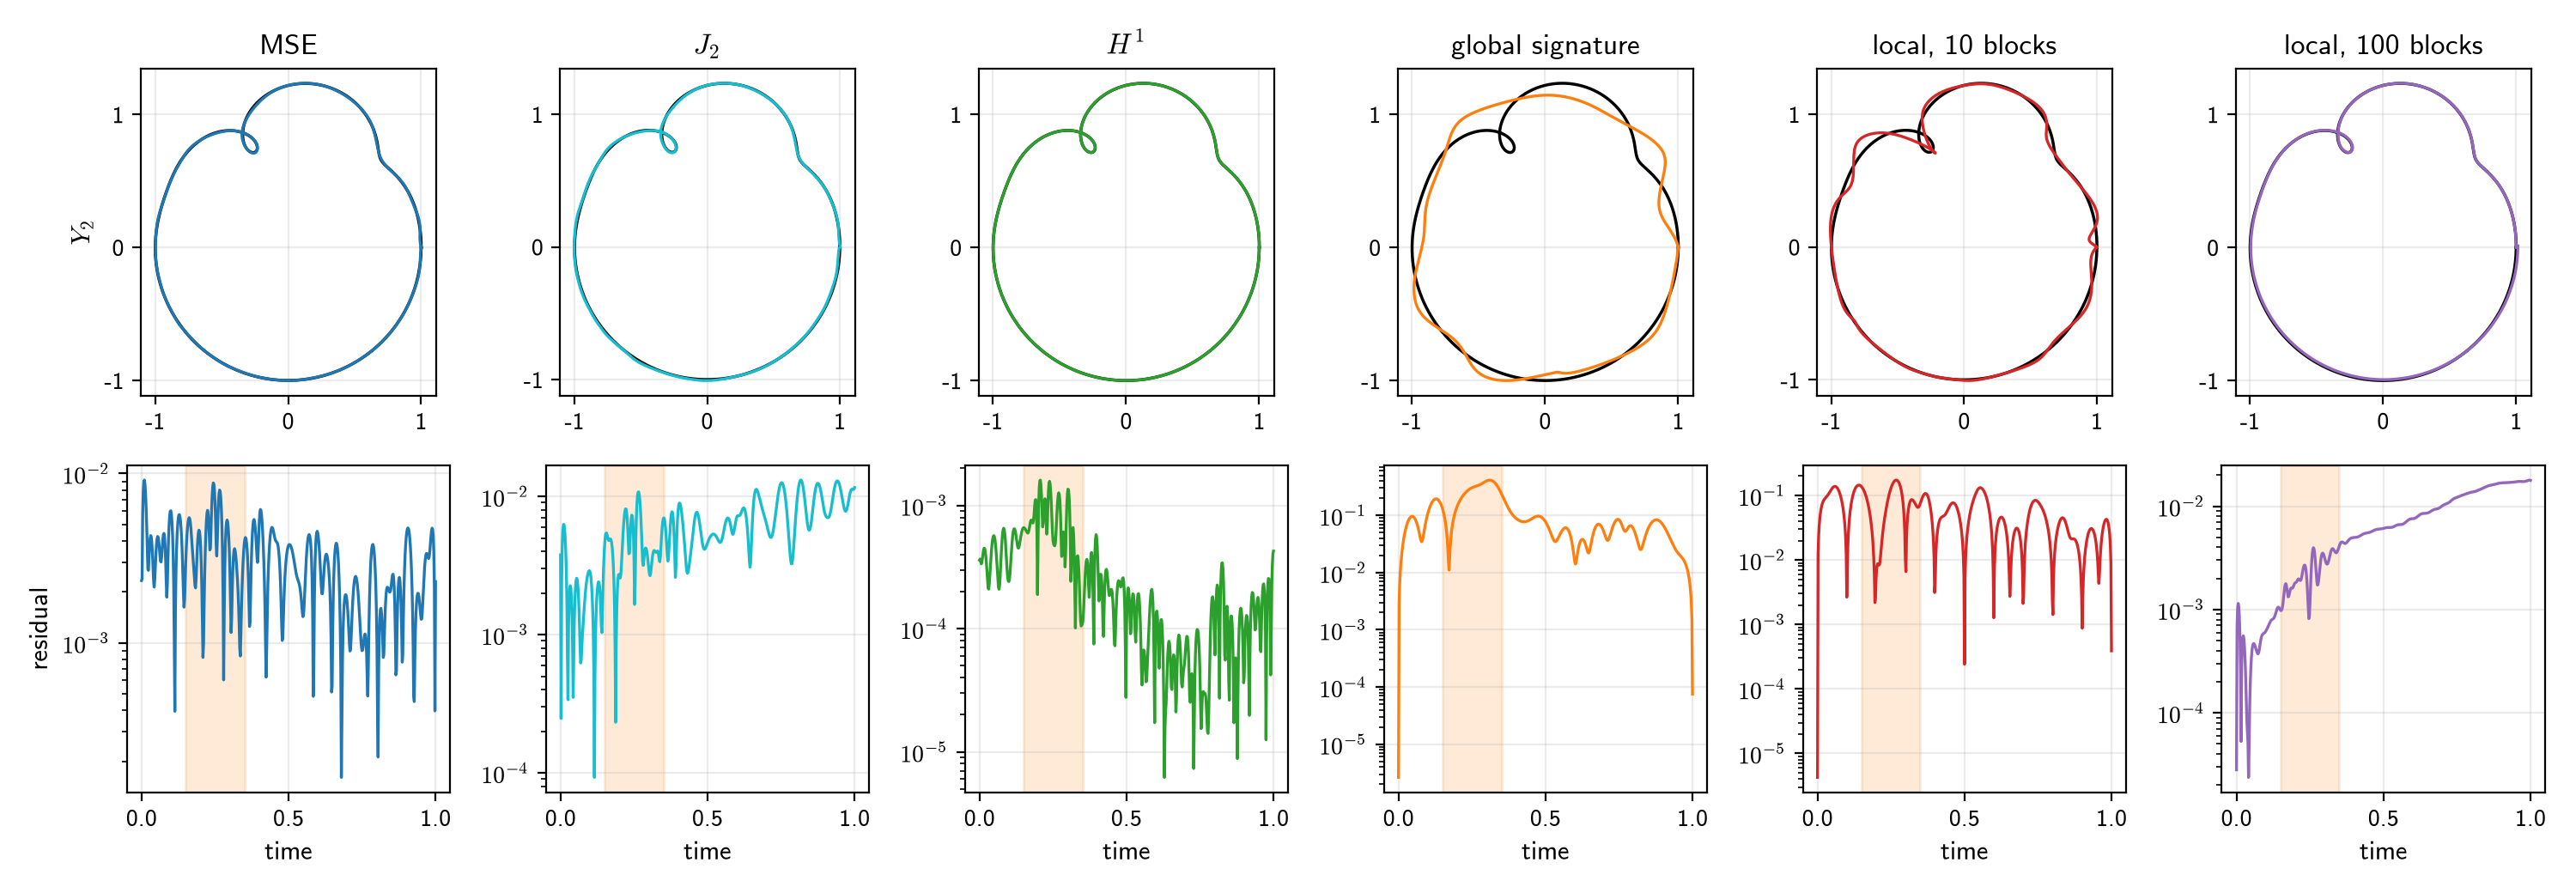
\includegraphics[width=\linewidth]{assets/fixed_terminal_restricted.png}
  \end{center}

  The upper row overlays the fitted path on the black target path. The lower row shows the residual magnitude over time, with the oscillatory burst shaded. All fits use seed 0, uniform observations and 10,000 Adam updates.
\end{frame}

\begin{frame}{Expressive-model terminal fits}
  \begin{center}
    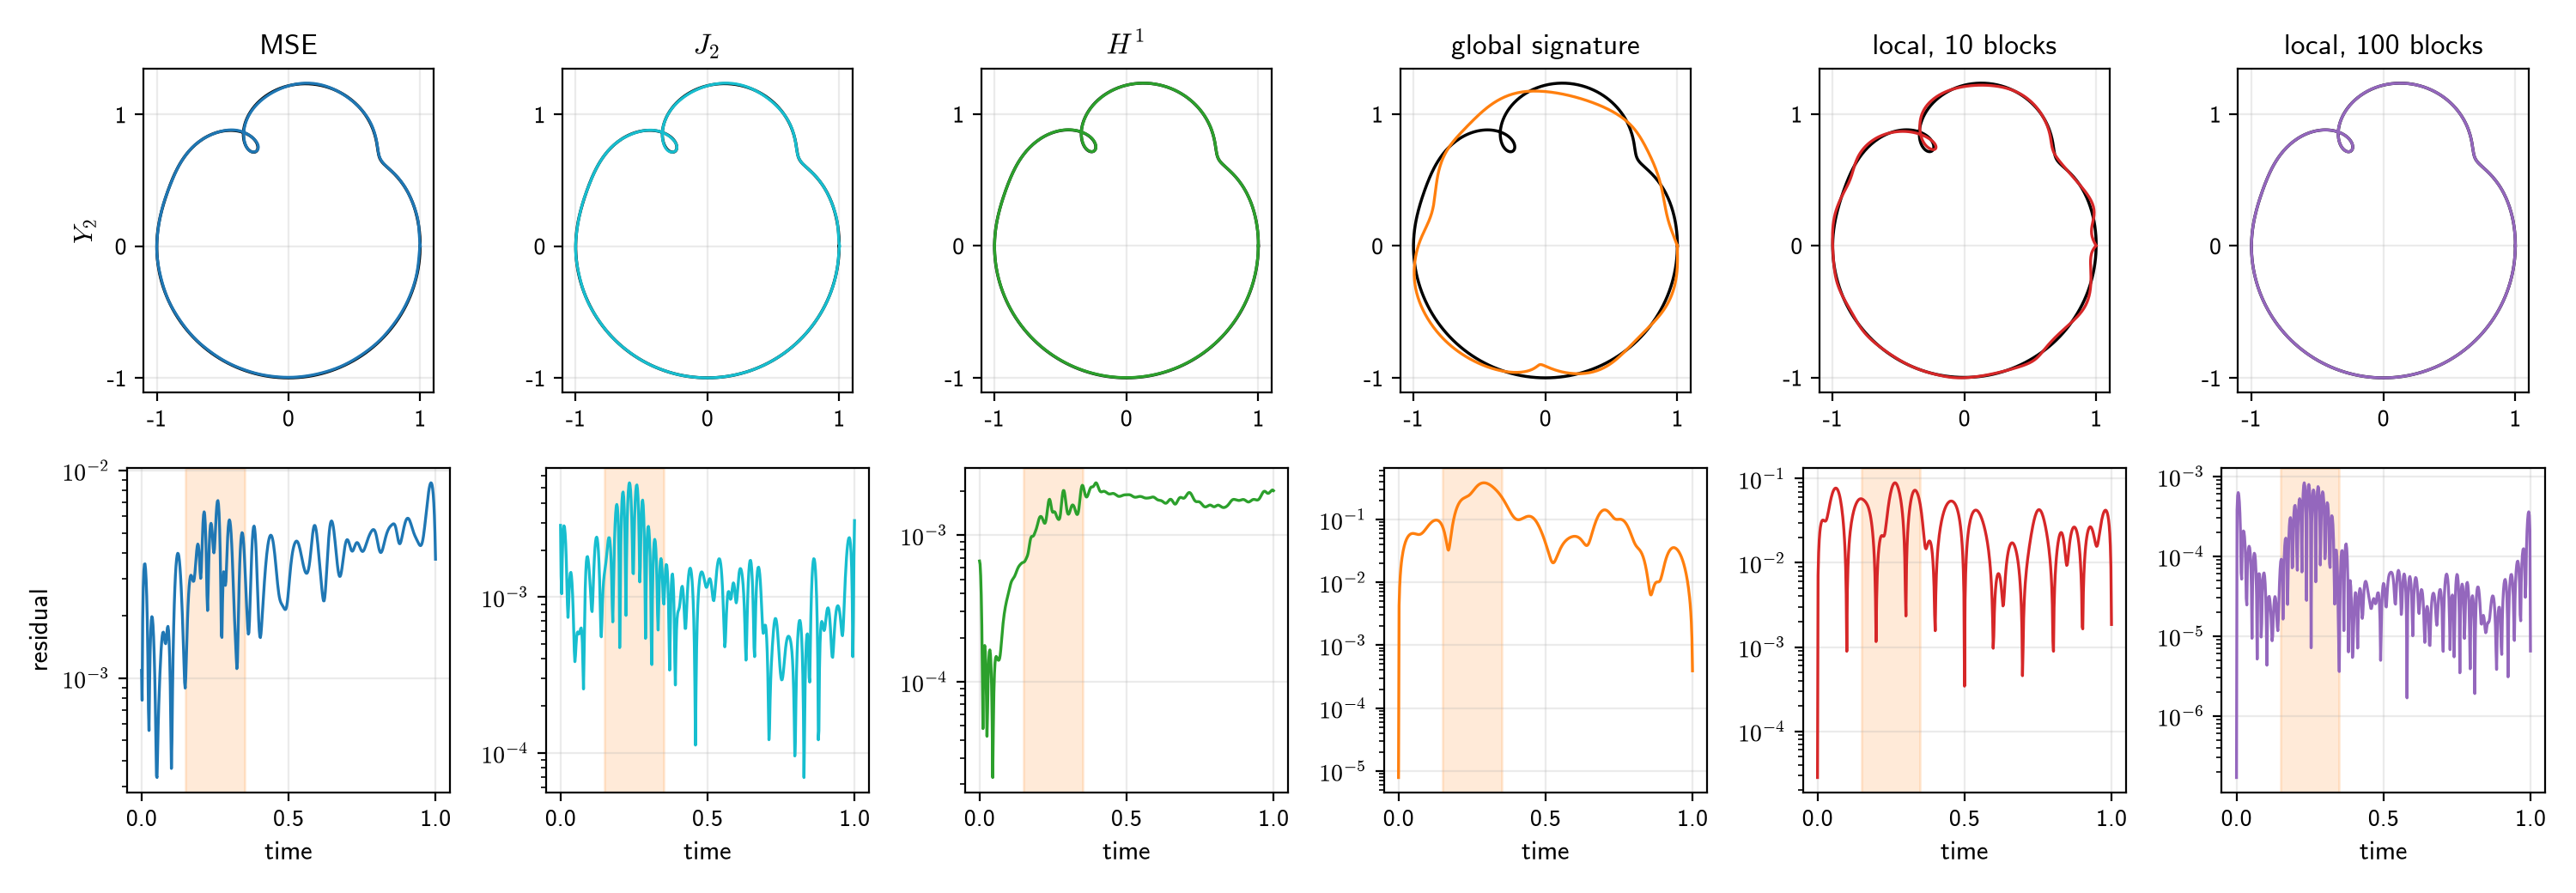
\includegraphics[width=\linewidth]{assets/fixed_terminal_expressive.png}
  \end{center}

  Extra capacity substantially improves the 10-block local-signature fit, while the global-signature fit remains limited by optimization under the common budget. The 100-block local-signature fit appears in the final column of both visual comparisons.
\end{frame}

\begin{frame}{Clustered-sampling residuals}
  \begin{center}
    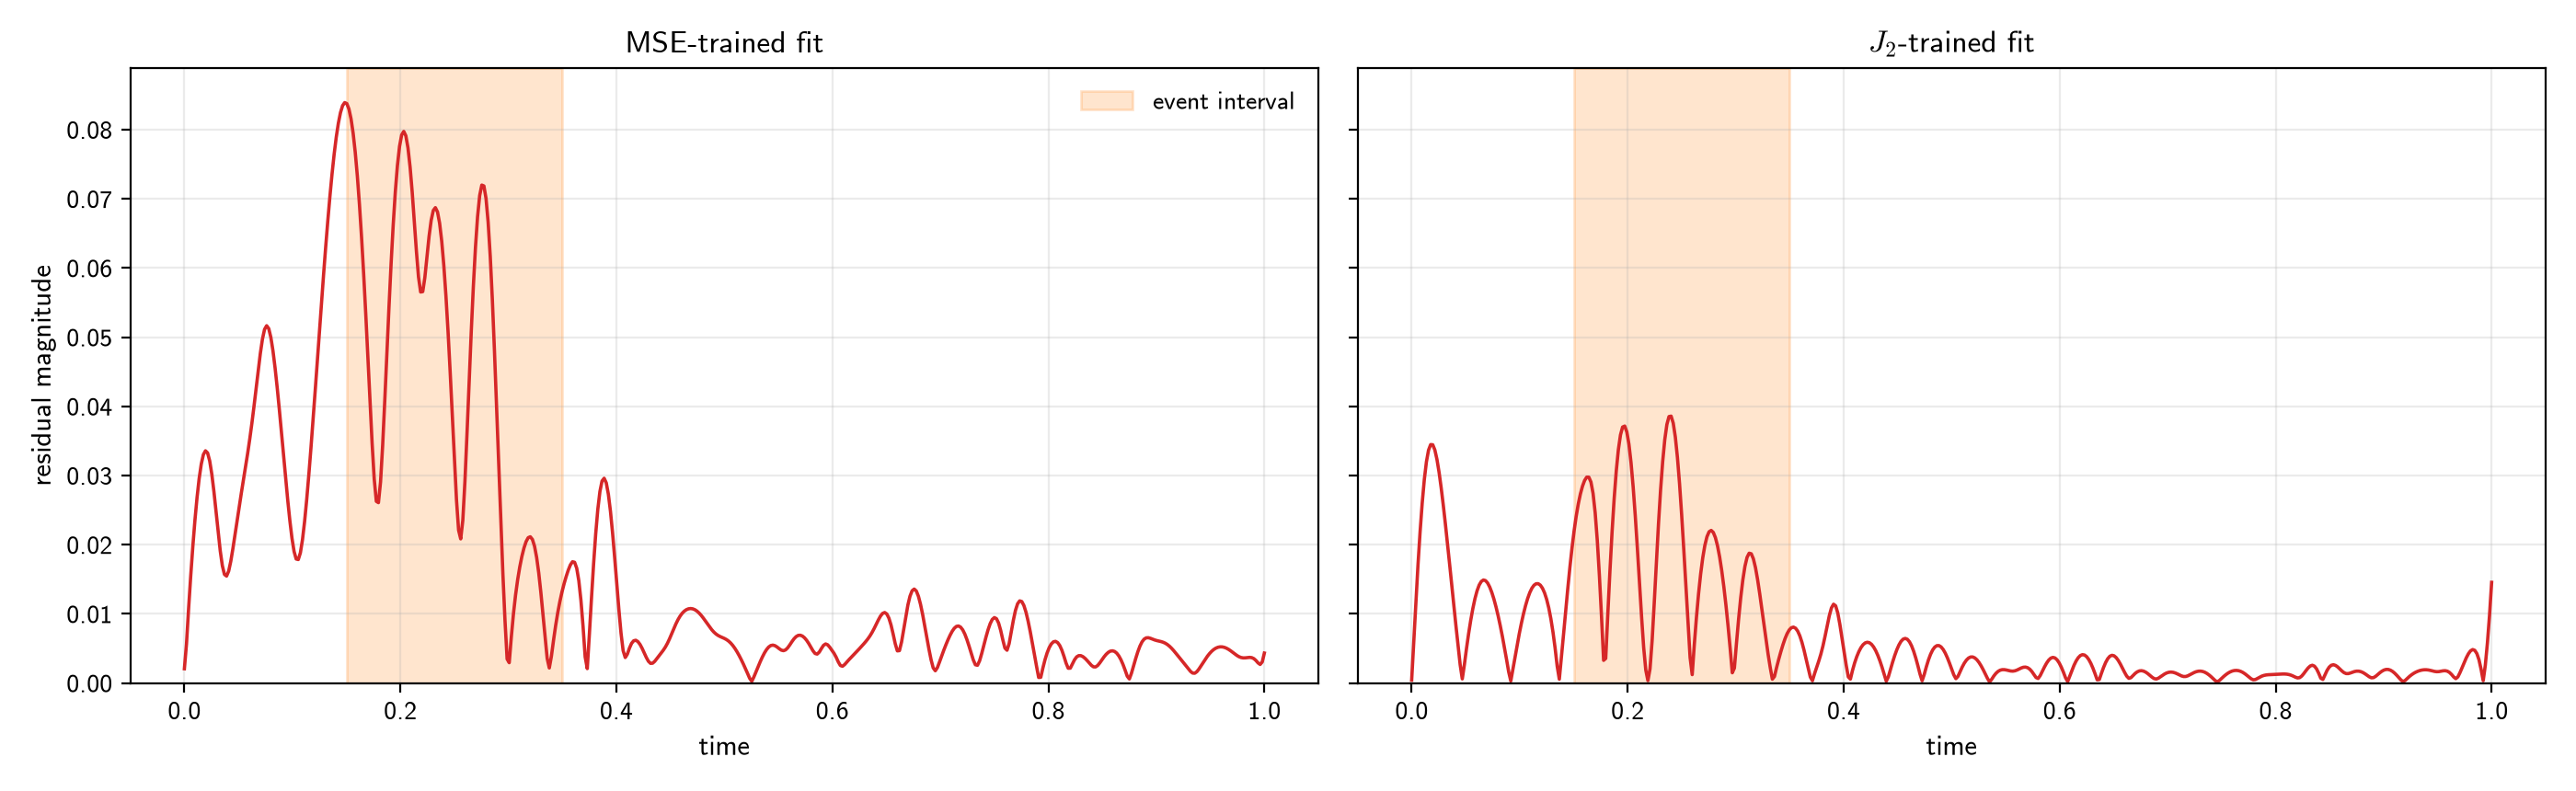
\includegraphics[width=\linewidth]{assets/fixed_clustered_residuals.png}
  \end{center}

  One matched restricted-model pair is shown. MSE gives equal weight to every recorded point, so the cluster receives disproportionate influence. The $\Jtwo$ quadrature weights instead approximate elapsed time and reduce error throughout the path.
\end{frame}

\begin{frame}{Sampling-density effect}
  Let $E^{\mathrm{MSE}}_{c,r}$ denote dense evaluation MSE for the model trained with MSE at capacity $c$ and seed $r$. Define $E^{\Jtwo}_{c,r}$ analogously for $\Jtwo$ training. With $R=3$ seeds, the reported ratio-of-means reduction is
  \[
    \operatorname{Reduction}_c
    :=1-
    \frac{R^{-1}\sum_{r=1}^{R}E^{\Jtwo}_{c,r}}
         {R^{-1}\sum_{r=1}^{R}E^{\mathrm{MSE}}_{c,r}}.
  \]
  Thus we first average the evaluation error across seeds for each training loss, then compare those two averages. This differs from calculating a percentage reduction within each seed and averaging the percentages.

  Under clustered sampling, $\Jtwo$ gives lower dense MSE in all six paired comparisons. The reduction is \result{68.4\%} for the restricted model and \result{40.8\%} for the expressive model. Under uniform sampling, each loss wins three of the six comparisons, as expected when the two objectives differ only through small endpoint-weight effects.
\end{frame}

\begin{frame}{Derivative supervision}
  $H^1$ training gives the best general errors in all six capacity-seed groups at update 1,000 and five of six groups at update 10,000. It directly penalizes velocity error, so it resolves the target's short oscillatory burst efficiently.

  This result depends on the smooth fixed target. Its derivative is known analytically, whereas Brownian paths are almost surely outside $H^1$. The same derivative supervision is therefore unavailable for rough stream tasks.

  Smooth targets can reward derivative-aware losses more than generic structural summaries. Signature losses are compared against this control rather than against MSE alone.
\end{frame}

\begin{frame}{Experiment A: learning dynamics}
  \begin{center}
    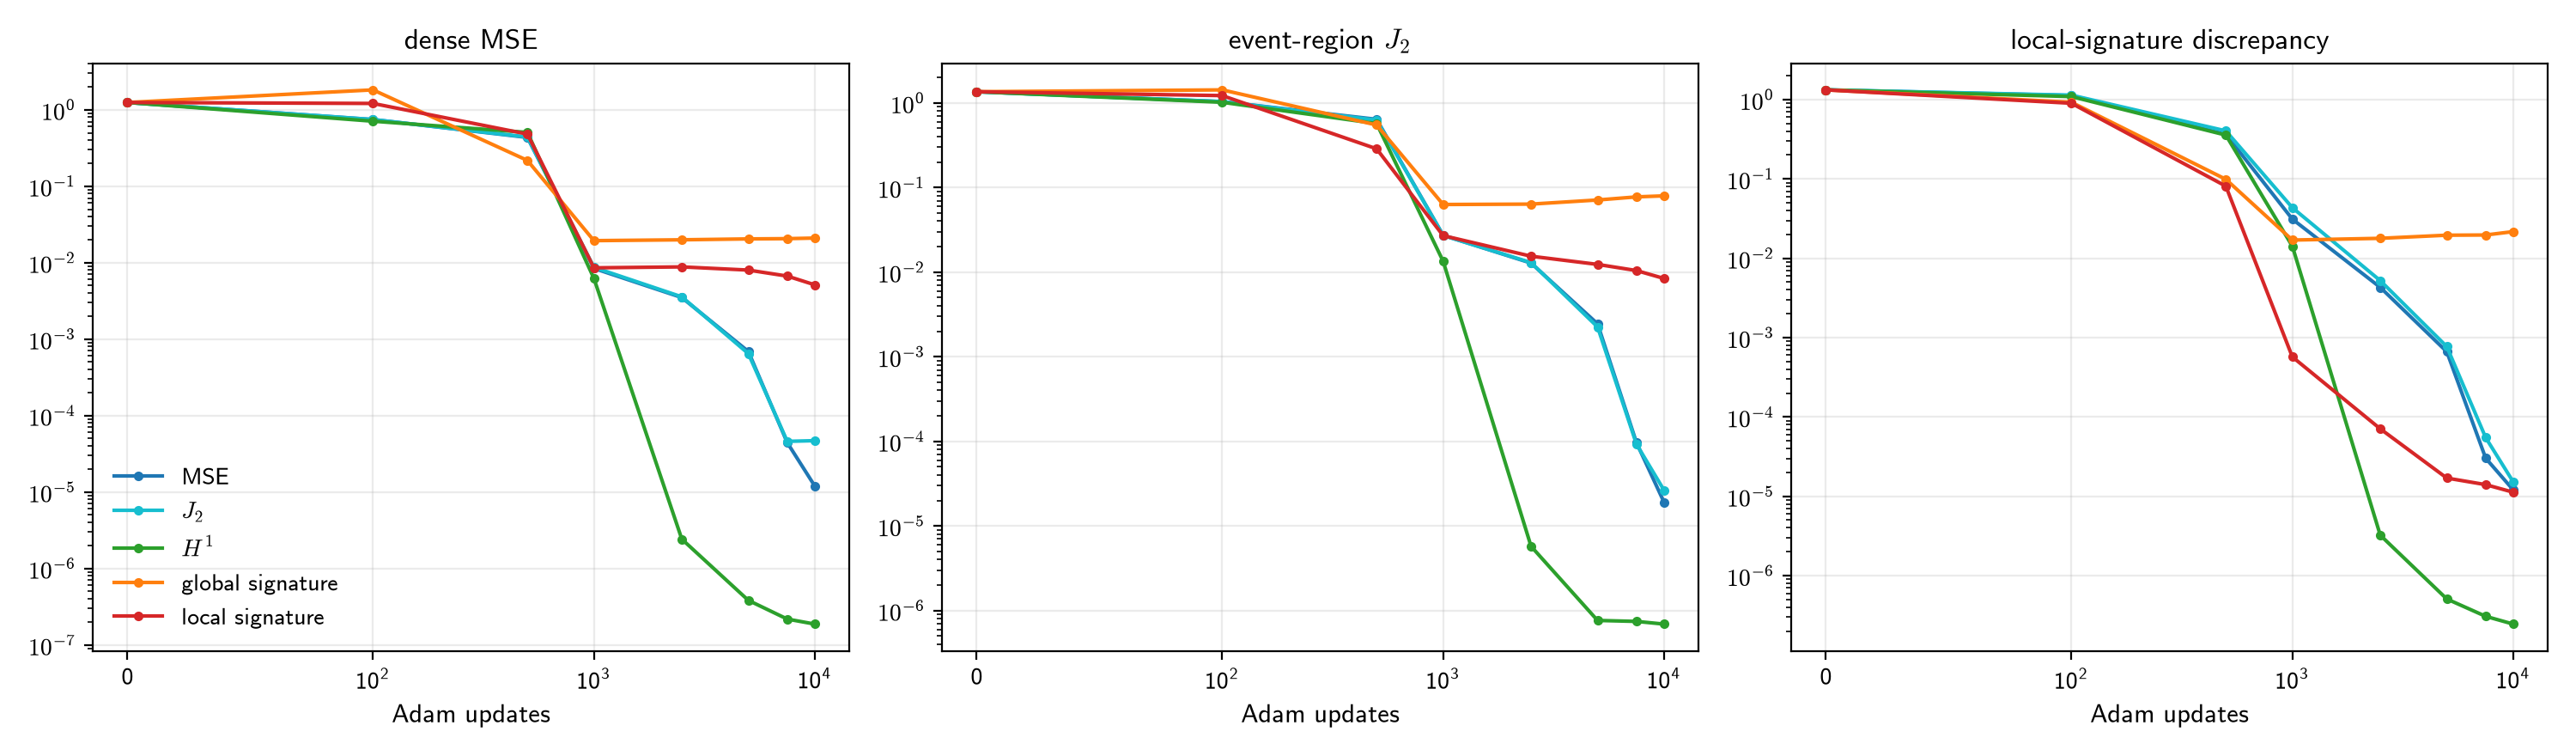
\includegraphics[width=\linewidth]{assets/learning_dynamics.png}
  \end{center}

  \vfill
  \begin{columns}[T,onlytextwidth]
    \begin{column}{0.47\textwidth}
      \textbf{Early advantage is objective-specific}\par
      At update 500 global-signature training leads on its own discrepancy in all six capacity-seed groups and local-signature training in five of six. Neither leads on event-region error, where pointwise and $H^1$ losses are ahead in five of six.
    \end{column}
    \begin{column}{0.47\textwidth}
      \textbf{Terminal fits alone would hide this}\par
      Signature advantage is transient. Reporting only update 10,000 would record a null where an ordering exists earlier in training.
    \end{column}
  \end{columns}
\end{frame}

\begin{frame}{Signature truncation and partition}
  \small
  \begin{center}
    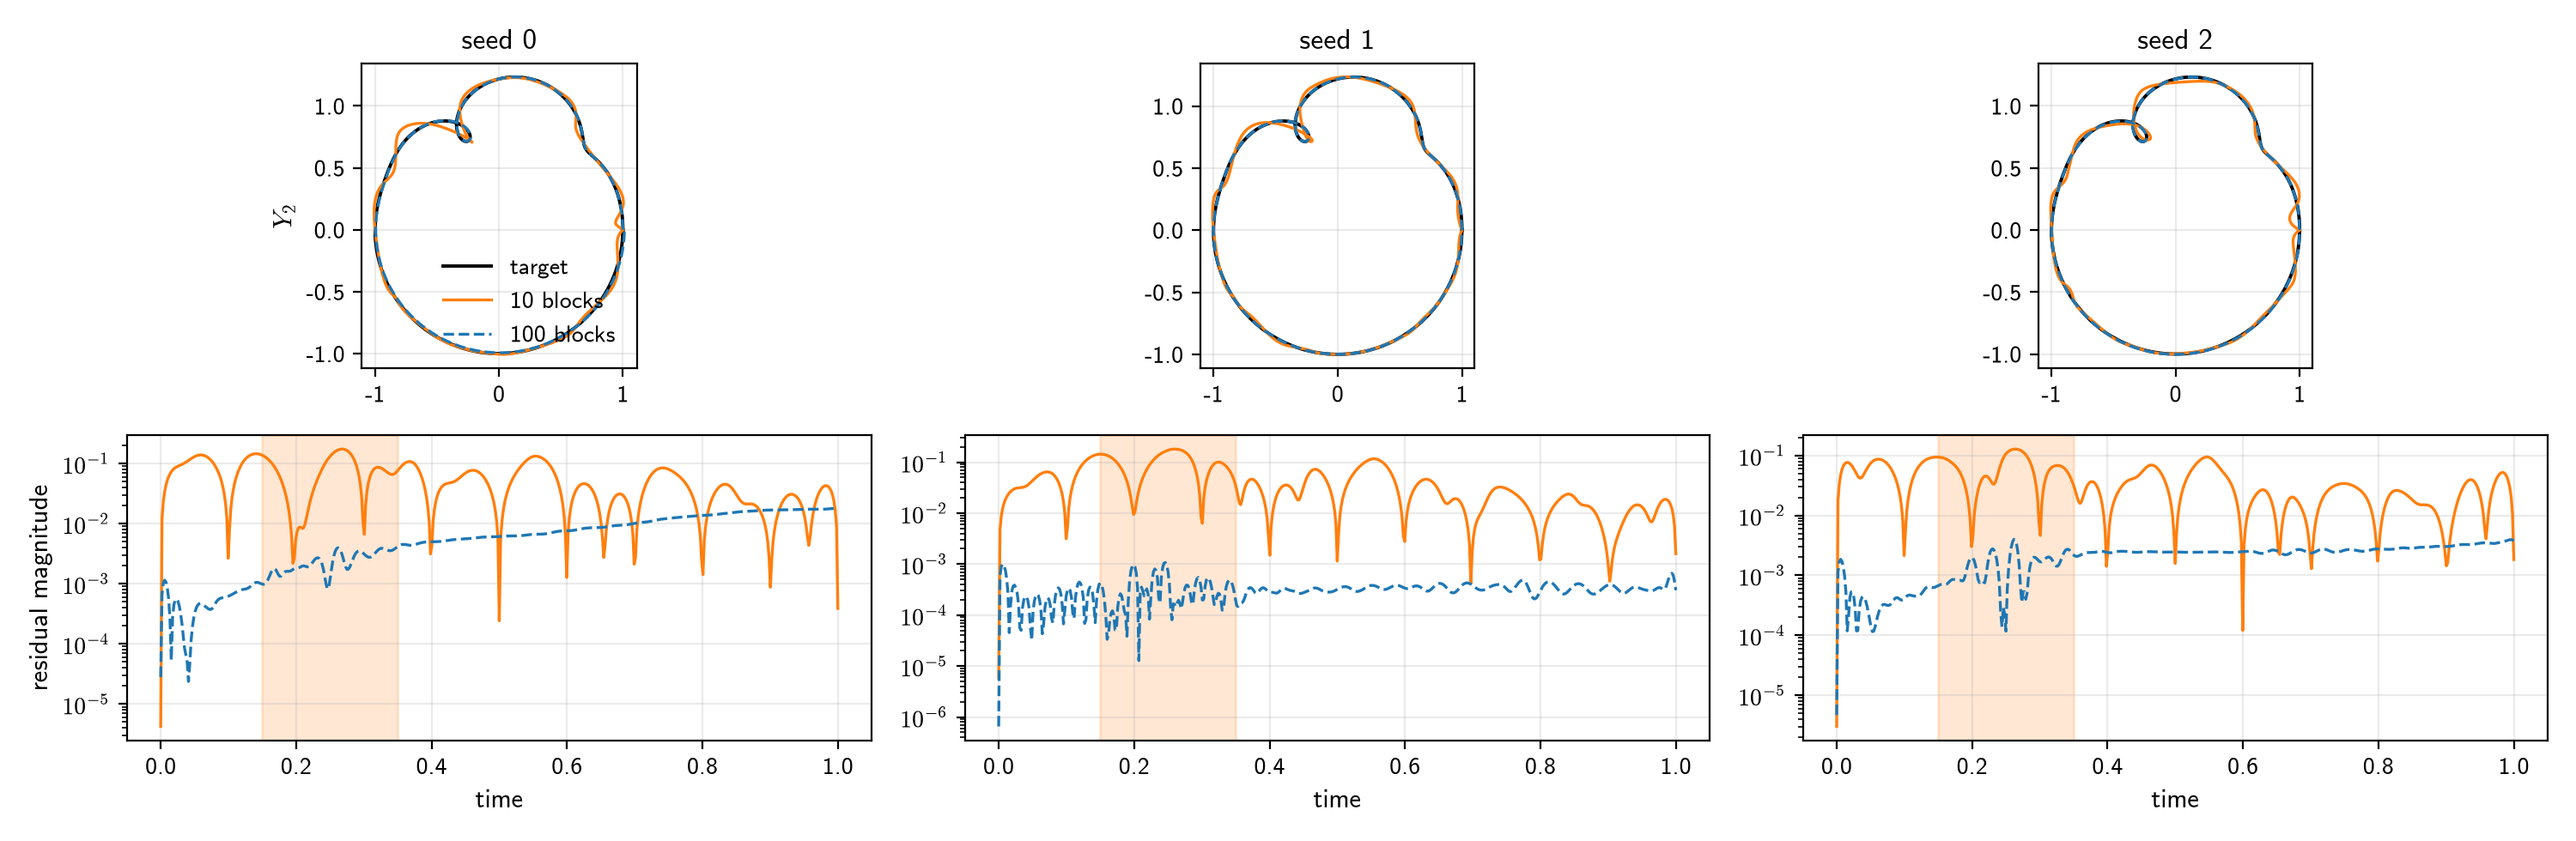
\includegraphics[width=\linewidth]{assets/path_comparison_restricted.png}
  \end{center}
  \begin{columns}[T,onlytextwidth]
    \begin{column}{0.47\textwidth}
      \textbf{Global depth 4}\par
      At the final update, pointwise-trained fits have lower global-signature error than the global-signature-trained fit in all six capacity-seed groups. Optimization limits this arm.
    \end{column}
    \begin{column}{0.47\textwidth}
      \textbf{Local depth 2}\par
      Refining the partition from 10 to 100 intervals lowers MSE, $\Jtwo$, $H^1$, maximum error and both local-signature discrepancies in all six capacity-seed groups.
    \end{column}
  \end{columns}
\end{frame}

\dividerframe{Experiment B: learned operator}

\begin{frame}{Experiment B: Brownian to OU}
  \begin{columns}[T,onlytextwidth]
    \begin{column}{0.47\textwidth}
      \textbf{Stream-to-stream task}\par
      A Brownian path $W$ drives an Ornstein--Uhlenbeck response $Y$:
      \[
        dY_t=-2Y_t\,dt+0.5\,dW_t,
        \qquad Y_0=0.
      \]
      Each input and target share the same Brownian increments. The model receives the whole driver path and returns the whole response path over the same interval.

      \textbf{Model}\par
      A Neural CDE learns the operator $\mathcal F_\theta:W\mapsto\widehat Y_\theta$ (Kidger et al., 2020):
      \[
        dh_t=f_\theta(h_t)\,d(t,W_t),
        \qquad \widehat Y_\theta(t)=g_\theta(h_t).
      \]
    \end{column}
    \begin{column}{0.47\textwidth}
      \textbf{Comparison}\par
      Separate models minimize MSE, $\Jtwo$, or a signature loss. Target times are uniform or clustered, while held-out evaluation always uses the full time grid.

      \textbf{Purpose}\par
      Experiment A fits one path. Experiment B tests whether the same loss effects persist when a single model must learn a map across many input and output paths.

      The comparison is matched: each loss sees the same paths, observation times, initialization, and training order.
    \end{column}
  \end{columns}
\end{frame}

\begin{frame}{Experiment B: operator learning}
  \begin{columns}[T,onlytextwidth]
    \begin{column}{0.39\textwidth}
      \textbf{Uniform target times}\par
      MSE and $\Jtwo$ give nearly identical held-out error. Equal point weights already approximate elapsed-time weighting.

      \textbf{Clustered target times}\par
      $\Jtwo$ lowers dense test $\Jtwo$ for all 3 paired seeds. Its across-seed mean is \result{51.7\% lower} than MSE training. Dense test MSE falls by 51.6\%.

      \textbf{Signature losses}\par
      Global-signature training is unstable across all 3 seeds. Local-signature training improves its own metric in 2 of 3 seeds, with one unstable run.
    \end{column}
    \begin{column}{0.57\textwidth}
      \centering
      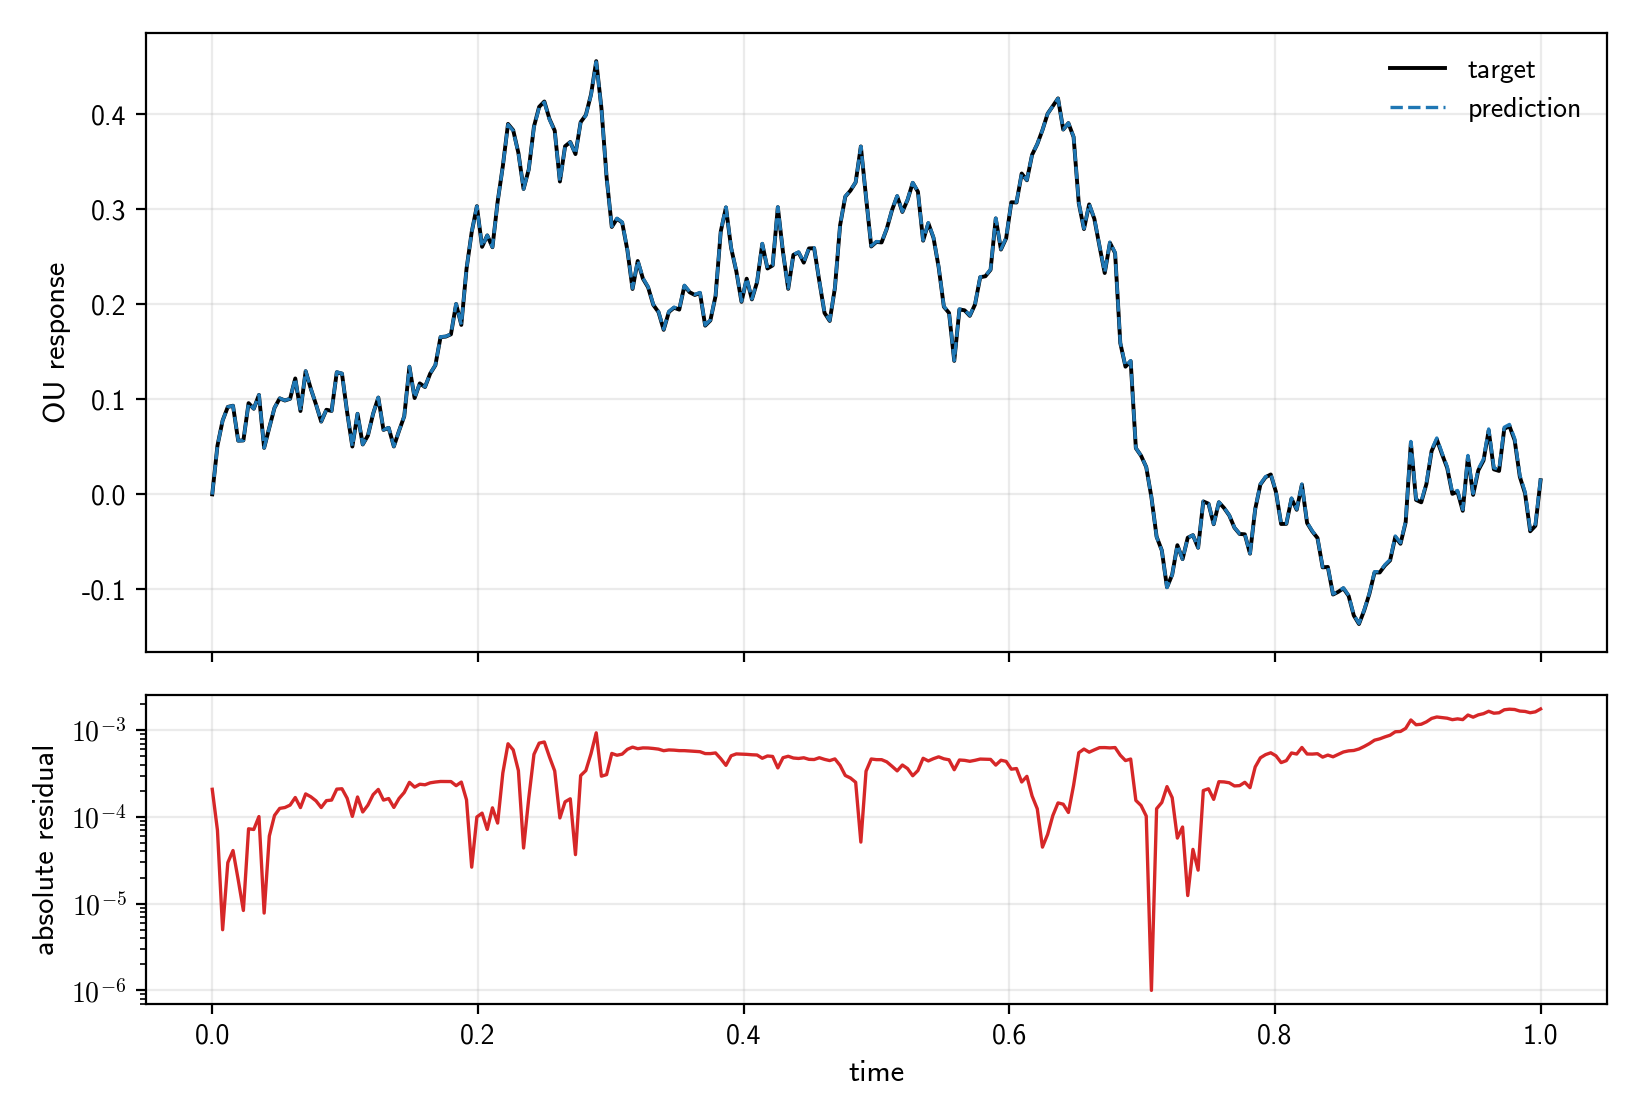
\includegraphics[width=\linewidth]{assets/ou_clustered_j2_response_path0.png}
      \par\scriptsize Clustered $\Jtwo$ fit, seed 1, held-out test path 0. Residual stays below $2\times10^{-3}$, so loss comparison concerns residual scale rather than shape.
    \end{column}
  \end{columns}
\end{frame}

\begin{frame}{Experiment B: optimizer stability}
  \begin{center}
    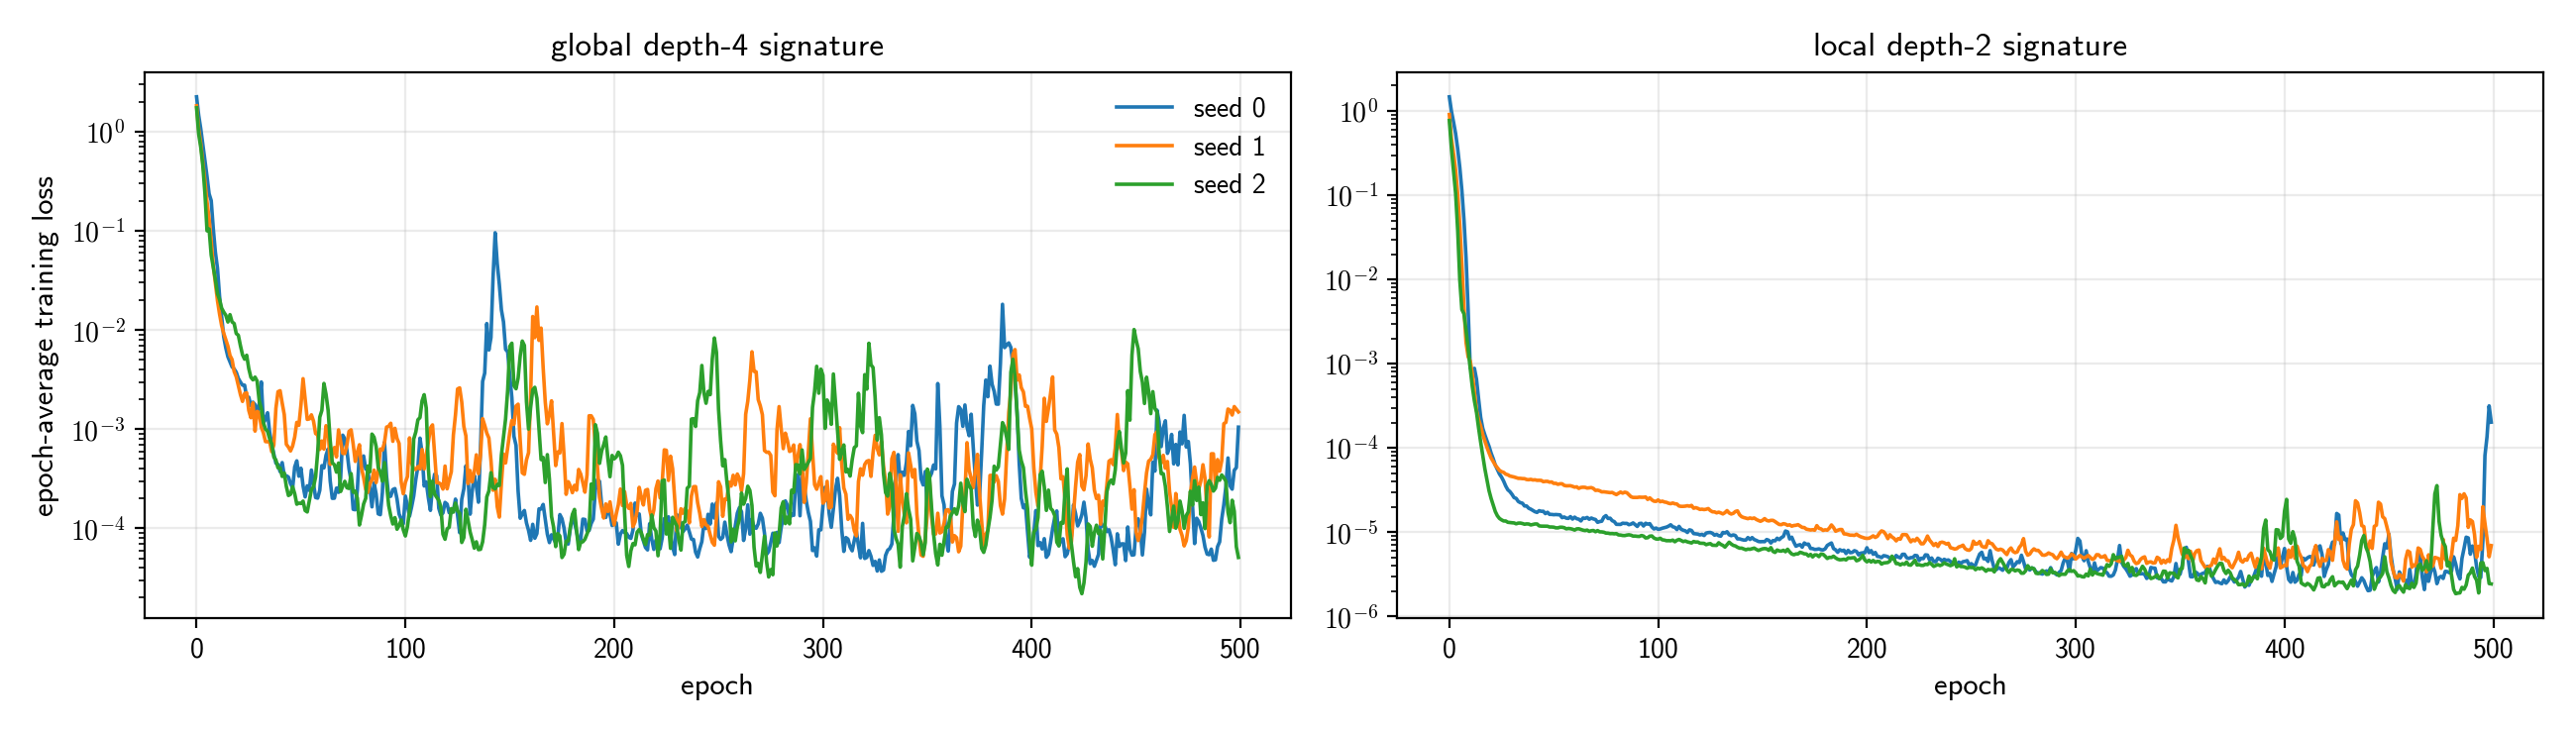
\includegraphics[width=\linewidth]{assets/ou_signature_histories.png}
  \end{center}

  \vfill
  Both signature objectives reach much lower training loss early, then rise. Final-to-best training-loss ratios are 28.4, 28.5 and 2.32 for the global loss. Terminal fits therefore record optimizer behaviour rather than a path the geometry prefers, so every signature claim in this project is stated at a fixed budget.
\end{frame}

\dividerframe{Experiment C: message sensitivity}

\begin{frame}{Experiment C: rough-path streams}
  Each supplied Brownian stream contains first-level increments and second-level L\'evy areas:
  \[
    X=\bigl((a_j,A_j)\bigr)_{j=0}^{2047},
    \qquad a_j\in\mathbb R^4,
    \quad A_j\in\Lambda^2\mathbb R^4.
  \]
  \begin{columns}[T,onlytextwidth]
    \begin{column}{0.46\textwidth}
      \textbf{Coordinate path}\par
      Cumulative sums of $a_j$ produce the visible four-dimensional path. MSE and integral norms compare this level.
    \end{column}
    \begin{column}{0.46\textwidth}
      \textbf{Rough-path lift}\par
      The six area coordinates $A_j$ retain within-step ordering that the coordinate path alone does not contain.
    \end{column}
  \end{columns}

  \textbf{Central construction}\par
  An area-only message changes $A_j$ while leaving every $a_j$ unchanged. Coordinate losses then return zero, whereas an appropriate rough-path distance can respond.

  The supplied simulation includes the joint Brownian area information. Independent Gaussian coordinate increments alone do not determine that information (Wiktorsson, 2001; Foster and Habermann, 2023).
\end{frame}

\begin{frame}{Experiment C: distances compared}
  Experiment C trains no path model. It measures how strongly each definition of distance responds to a controlled message.

  \begin{tabular}{>{\bfseries}p{0.20\textwidth}p{0.38\textwidth}p{0.32\textwidth}}
    \toprule
    Path view & Examples & Information available \\
    \midrule
    Coordinate & MSE, integral norms, maximum error & Visible coordinate motion \\
    Rough path & Direct area distance & Stored second-level area \\
    Global signature & Signature through depth four & Overall ordered structure \\
    Local signature & Depth two on short intervals & Approximate location of structure \\
    Derived signature & Variance-normalized and response-derived distances & Alternative weighting of signature levels \\
    \bottomrule
  \end{tabular}

  \vfill
  Variance normalization puts naturally small higher levels on a comparable scale. Comparing aligned and shifted local partitions tests whether sensitivity depends on where interval boundaries fall.
\end{frame}

\begin{frame}{Experiment C: variance-normalized signature distance}
  For block $b$ and signature level $k$, define
  \[
    \Delta S_b^{(k)}(X,Y):=S_b^{(k)}(X)-S_b^{(k)}(Y).
  \]
  Let $q_k^2$ be the empirical training variance per level-$k$ coordinate, averaged over streams and blocks. Since a four-dimensional level-$k$ signature has $4^k$ coordinates, set
  \[
    d_{\mathrm{var}}(X,Y)
    :=\left[
      \frac1B\sum_{b=1}^{B}\sum_{k=1}^{L}
      \frac{\|\Delta S_b^{(k)}(X,Y)\|_2^2}
           {4^k(q_k^2+\delta)}
    \right]^{1/2},
    \qquad \delta=10^{-12}.
  \]

  \textbf{Motivation for the weights}\par
  Factor $4^{-k}$ averages over coordinates. Division by $q_k^2$ measures a discrepancy relative to the natural Brownian variation at that level. The small constant $\delta$ only protects against division by zero.

  The global version uses one block through depth four. Local versions use depth two over short aligned or shifted blocks.
\end{frame}

\begin{frame}{Experiment C: response-derived signature distance}
  In a linear controlled differential equation, a level-$k$ signature coordinate is multiplied by a product of $k$ response matrices. If every matrix satisfies $\|A_i\|_{\mathrm{op}}\le r$, then
  \[
    \|A_{i_k}\cdots A_{i_1}\|_{\mathrm{op}}
    \le \prod_{j=1}^{k}\|A_{i_j}\|_{\mathrm{op}}
    \le r^k.
  \]
  This motivates the response-derived discrepancy
  \[
    U_{r,L}(X,Y)
    :=\frac1B\sum_{b=1}^{B}\sum_{k=1}^{L}
      r^k\|\Delta S_b^{(k)}(X,Y)\|_1.
  \]

  Parameter $r$ represents the scale of the response system. Small $r$ suppresses higher levels; large $r$ makes them more influential. The experiment uses $r\in\{0.5,1,2\}$. The coordinate $\ell^1$ norm matches the sum of absolute signature contributions produced by the triangle-inequality bound.

  Thus $U_{r,L}$ estimates how distinguishable two streams could be through a family of linear responses. It is a project discrepancy motivated by the response bound of Ferrucci, Perr\'ee and Lyons (2026), rather than a canonical signature metric.
\end{frame}

\begin{frame}{Experiment C: sensitivity tests}
  \begin{columns}[T,onlytextwidth]
    \begin{column}{0.47\textwidth}
      \textbf{Paired response}\par
      Compare each original stream with its own modified copy. Normalize this distance by the typical distance between unrelated Brownian streams.

      This shows whether a message is visible relative to ordinary variation in the data.
    \end{column}
    \begin{column}{0.47\textwidth}
      \textbf{Single-stream detection}\par
      A one-nearest-neighbour classifier uses one distance at a time to separate original and modified streams.

      The smallest reliably detectable amplitude gives a practical sensitivity threshold. A second independent ensemble checks whether every selected threshold repeats.
    \end{column}
  \end{columns}

  \vfill
  Together, the two views distinguish a metric that merely changes numerically from one that can identify a weak message in a population of random streams.
\end{frame}

\begin{frame}{Experiment C: message construction}
  \small
  A message modifies 16 increments near the middle of a stream. Its amplitude $\rho$ is measured in units of the natural Brownian scale.

  \begin{tabular}{>{\bfseries}p{0.18\textwidth}p{0.28\textwidth}p{0.44\textwidth}}
    \toprule
    Message & Modified component & Intended probe \\
    \midrule
    Increment & First-level increments & Visible coordinate displacement \\
    Area & Second-level areas & Hidden information with no coordinate change \\
    Combined & Both levels & Mixed coordinate and area information \\
    \midrule
    Net template & All perturbations have the same sign & Accumulated change and endpoint displacement \\
    Balanced template & Eight positive, then eight negative & Local ordering with zero direct sum \\
    \bottomrule
  \end{tabular}
  Amplitudes range from an exact zero-message control to several times the natural scale. The rough-path composition law keeps every modified stream algebraically consistent.
\end{frame}

\begin{frame}{Experiment C: message templates}
  \begin{center}
    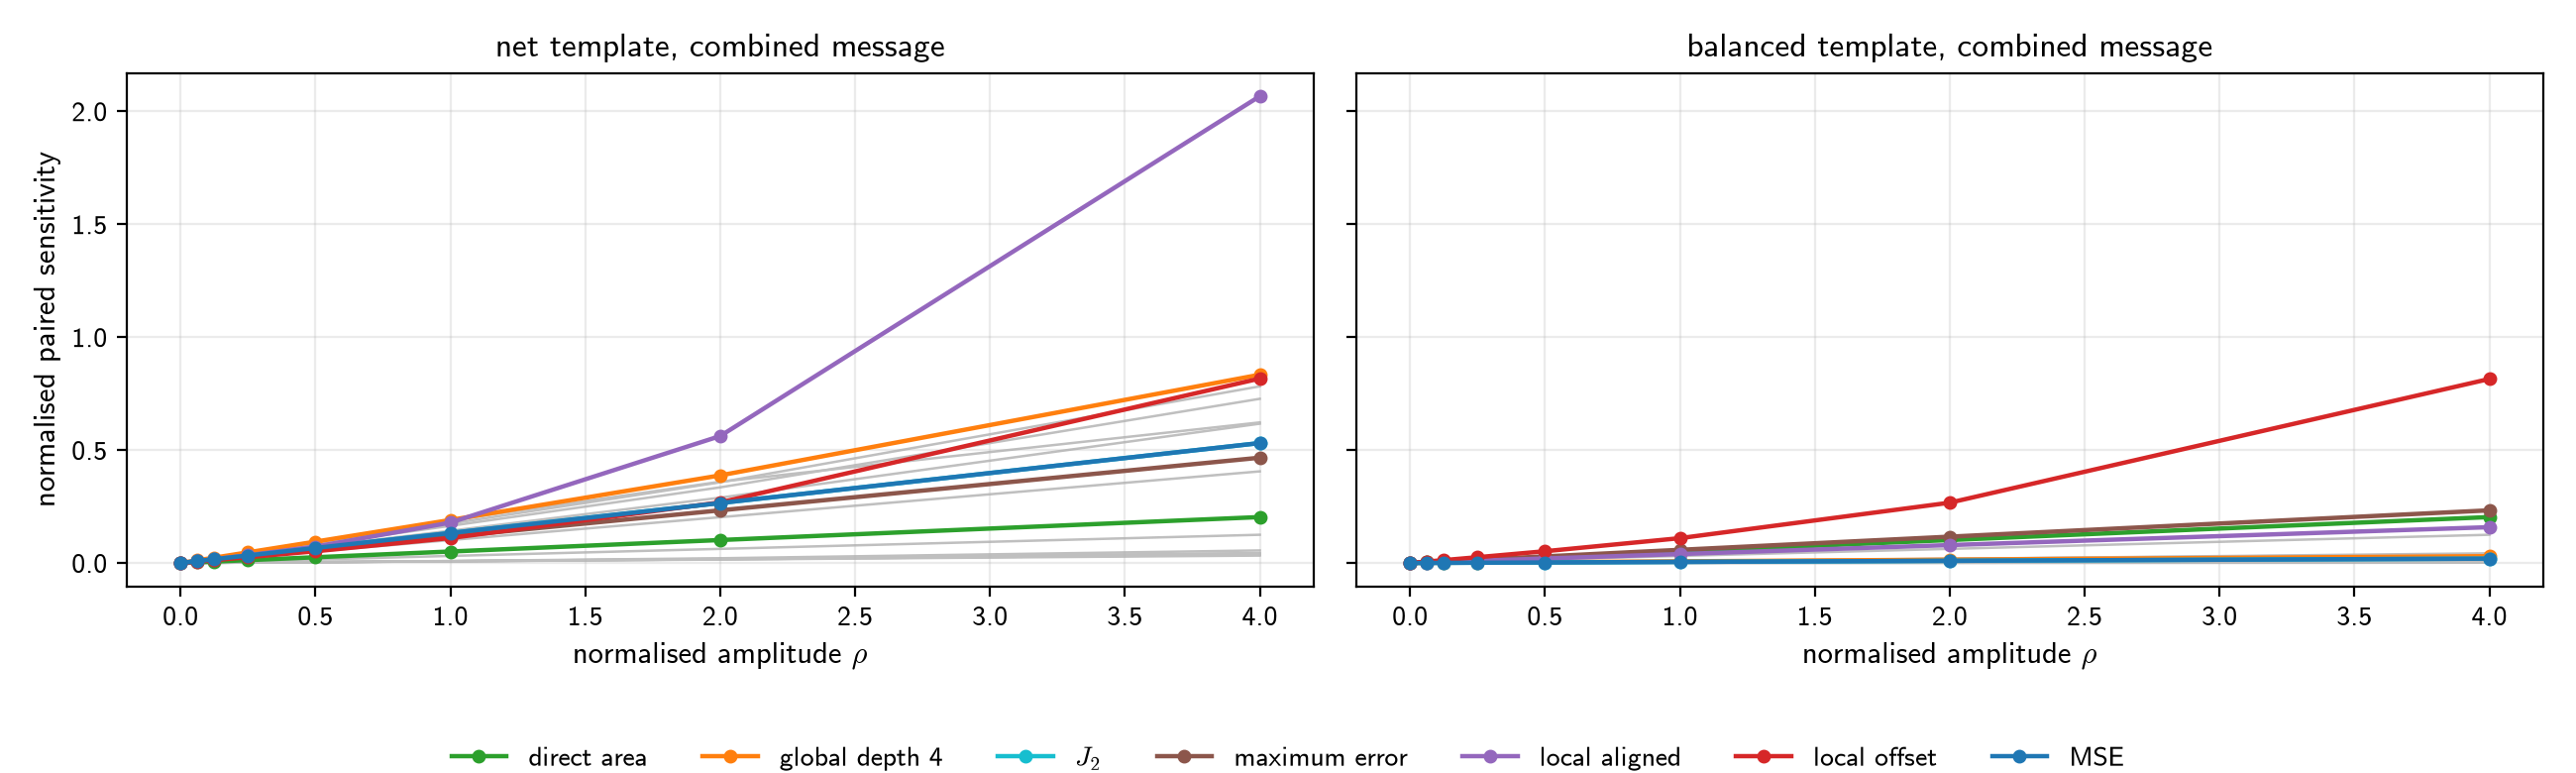
\includegraphics[width=\linewidth]{assets/template_comparison.png}
  \end{center}

  \vfill
  \begin{columns}[T,onlytextwidth]
    \begin{column}{0.47\textwidth}
      \textbf{Net template}\par
      Inserted increments accumulate, so endpoint displacement alone separates the classes and every discrepancy responds.
    \end{column}
    \begin{column}{0.47\textwidth}
      \textbf{Balanced template}\par
      Direct increments sum to zero over the block. Response now depends on whether a representation retains local order, which is the discriminating case.
    \end{column}
  \end{columns}
\end{frame}

\begin{frame}{Experiment C: balanced messages}
  \centering
  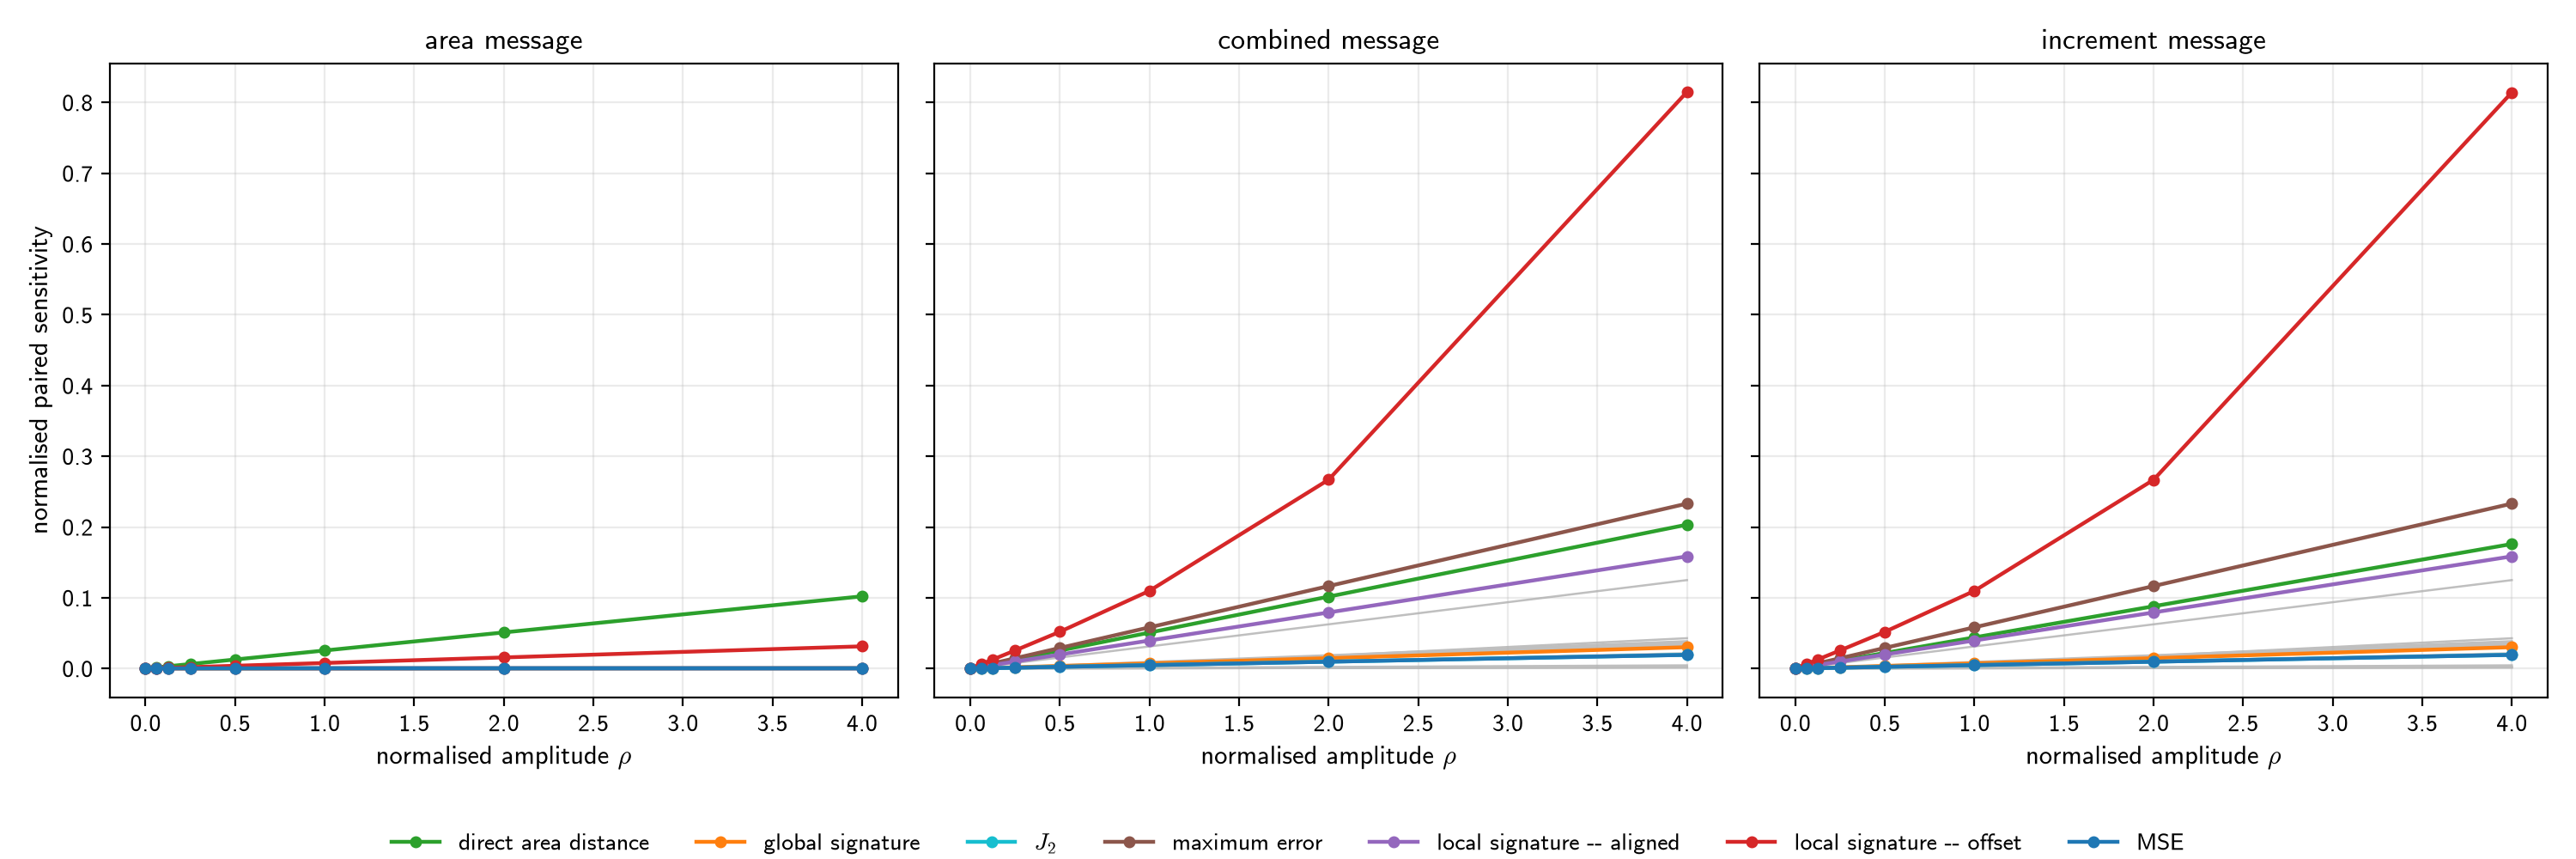
\includegraphics[width=\linewidth]{assets/paired_balanced.png}
  \small
  \begin{columns}[T,onlytextwidth]
    \begin{column}{0.31\textwidth}
      \textbf{Area only}\par
      Coordinate losses remain zero because $a_j$ is unchanged. Area and signature features respond.
    \end{column}
    \begin{column}{0.31\textwidth}
      \textbf{Combined}\par
      Offset local signatures amplify a message whose direct increments cancel over the full block.
    \end{column}
    \begin{column}{0.31\textwidth}
      \textbf{Increment only}\par
      Pointwise losses respond to the local excursion. Signature response depends on partition placement.
    \end{column}
  \end{columns}
\end{frame}

\begin{frame}{Experiment C: partition alignment}
  \small
  \begin{columns}[T,onlytextwidth]
    \begin{column}{0.47\textwidth}
      \textbf{Aligned local signature}\par
      A comparison interval contains the full balanced message. Added level-one increments and direct level-two areas sum to zero, so depth two can cancel.
    \end{column}
    \begin{column}{0.47\textwidth}
      \textbf{Offset local signature}\par
      A boundary cuts through the message. Partial sums no longer cancel inside each interval, creating a deterministic depth-two response.
    \end{column}
  \end{columns}
  \begin{center}
  \begin{tikzpicture}[x=0.105cm,y=0.58cm]
    % message sits inside one aligned block [32,64] and is cut by offset boundary 48
    \draw[very thick,oxfordblue] (0,0) -- (128,0);
    \foreach \x in {0,32,64,96,128}{\draw[oxfordblue] (\x,-0.18)--(\x,0.18);}
    \fill[oxfordblue!55] (40,-0.09) rectangle (56,0.09);
    \node[above,black] at (48,0.24) {balanced message};
    \node[below,oxfordblue] at (96,-0.26) {aligned blocks: message intact};
    \draw[very thick,dashed,darkgrey] (16,-1.30) -- (112,-1.30);
    \foreach \x in {16,48,80,112}{\draw[darkgrey] (\x,-1.48)--(\x,-1.12);}
    \fill[oxfordblue!55] (40,-1.39) rectangle (56,-1.21);
    \draw[darkgrey,thick] (48,-1.52)--(48,-1.08);
    \node[below,darkgrey] at (96,-1.54) {offset blocks: boundary cuts message};
  \end{tikzpicture}
  \end{center}
  \centering Partition choice is part of the loss definition.
\end{frame}

\begin{frame}{Experiment C: single-stream detection}
  \begin{center}
    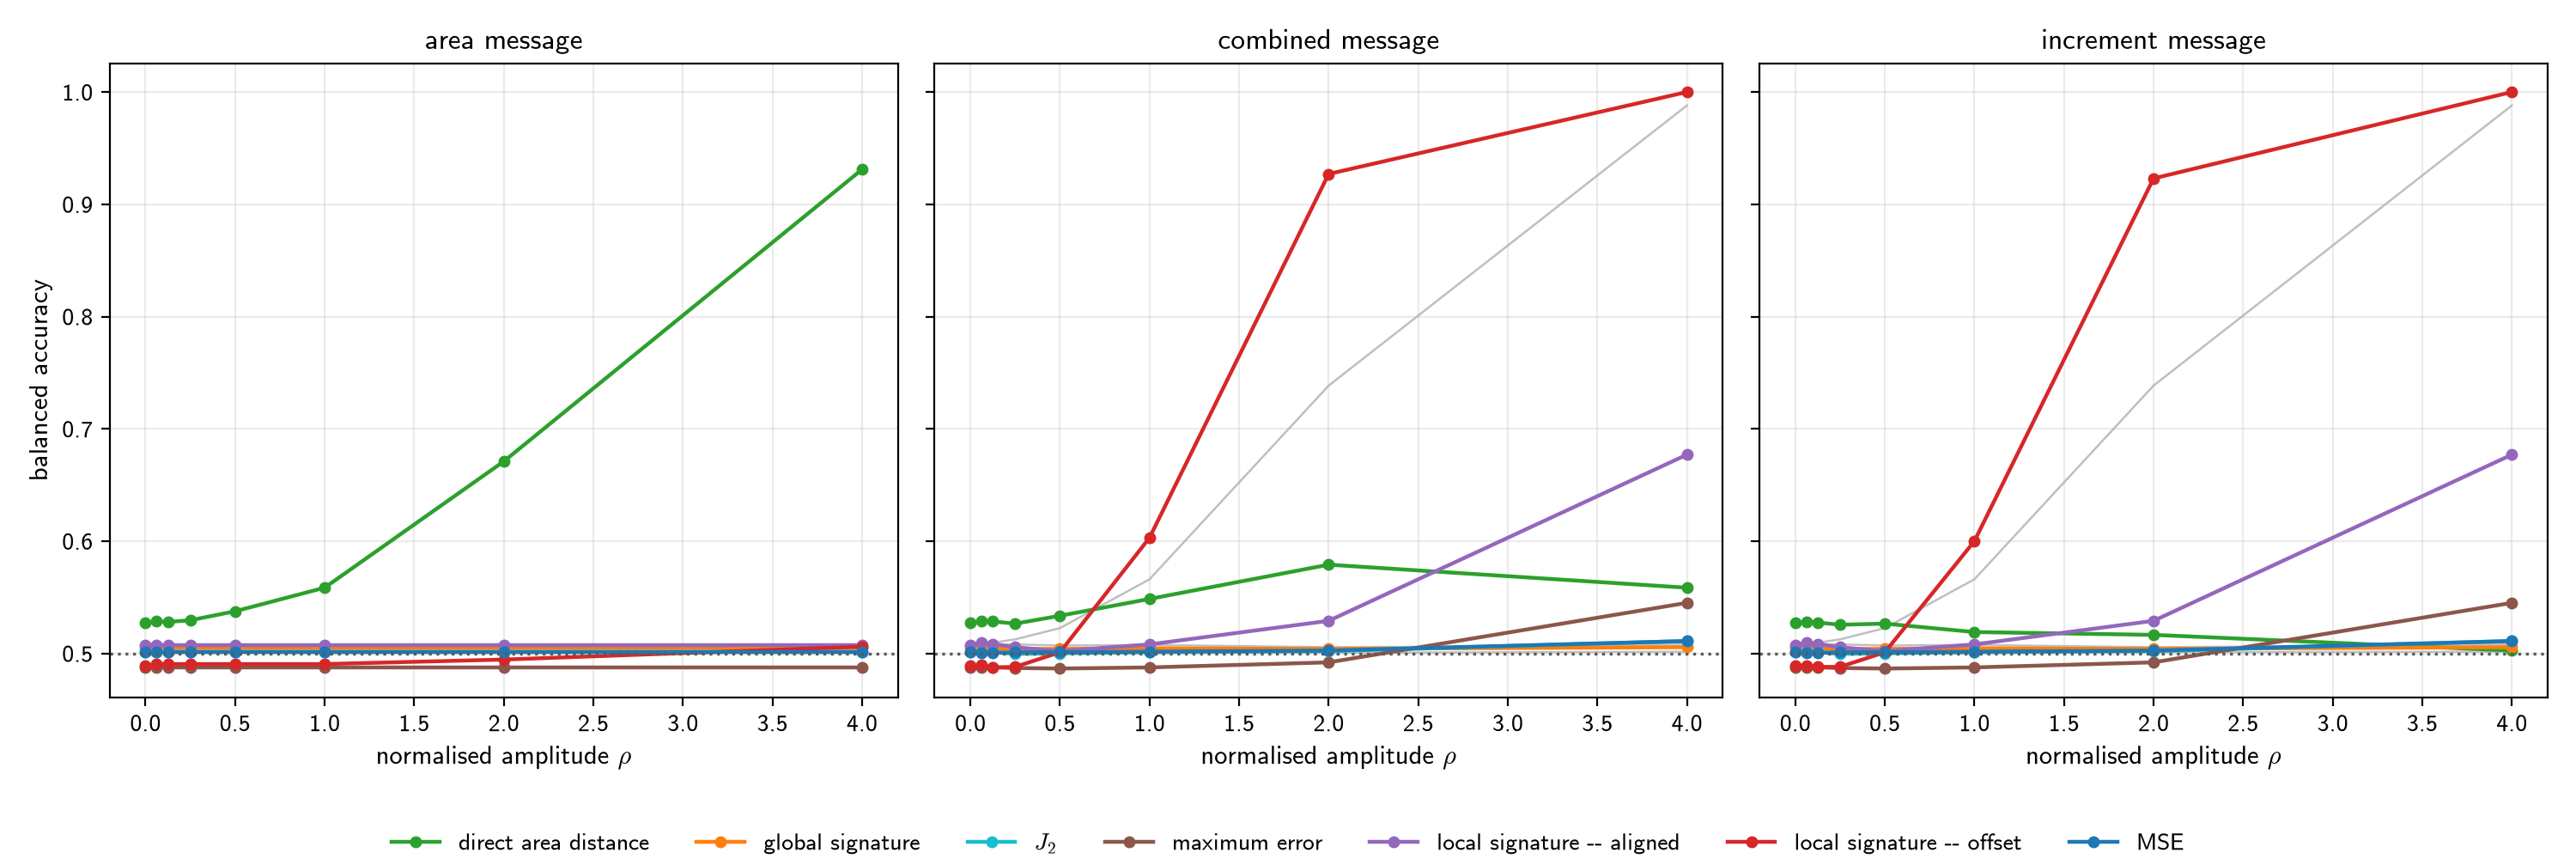
\includegraphics[width=\linewidth]{assets/detection_balanced.png}
  \end{center}
  \small
  Classifier $\widehat c_d$ uses one loss-derived distance $d$; the dotted line marks chance balanced accuracy $\operatorname{BA}=1/2$. For balanced increment and combined messages, direct increment features detect from $\rho=0.5$, offset local signatures from $\rho=1$, aligned local signatures from $\rho=2$, and maximum error from $\rho=4$. Every transition reproduces on the independent confirmation ensemble.
\end{frame}

\dividerframe{Conclusions}

\begin{frame}{Summary}
  \small
  \begin{tabular}{>{\bfseries}p{0.22\textwidth}p{0.31\textwidth}p{0.37\textwidth}}
    \toprule
    Evidence & Main result & Meaning of closeness \\
    \midrule
    Sampling limit & MSE targets a density-weighted integral & Observation frequency \\
    Fixed path and OU & $\Jtwo$ corrects clustered bias & Elapsed time \\
    Smooth fixed path & $H^1$ resolves a short oscillatory burst & Values and derivatives \\
    Brownian messages & Signature features detect area and order & Ordered multilevel structure \\
    \bottomrule
  \end{tabular}
  \textbf{Project conclusion}\par
  Two paths count as close only relative to structure relevant to the task. Observation density, regularity, scale, signature truncation, localization and optimization can each change the comparison.
\end{frame}

\begin{frame}{Scope and continuation}
  \begin{columns}[T,onlytextwidth]
    \begin{column}{0.47\textwidth}
      \textbf{Supported conclusions}\par
      \begin{itemize}
        \item Use elapsed-time weights under irregular sampling.
        \item Use derivative penalties when smooth derivatives are meaningful.
        \item Use signature features when order or area matters.
        \item Treat signature partition and scaling as model choices.
      \end{itemize}
    \end{column}
    \begin{column}{0.47\textwidth}
      \textbf{Scope}\par
      One fixed target, one operator, one Brownian law, finite training budgets and three seeds. Signature training remains sensitive to optimization.

      \textbf{Natural continuation}\par
      Hybrid losses, multiscale local signatures, learned path representations and broader stream operators.
    \end{column}
  \end{columns}
\end{frame}

\begin{frame}{Appendix: Experiment A comparison matrix}
  \small
  \begin{columns}[T,onlytextwidth]
    \begin{column}{0.46\textwidth}
      \begin{block}{Training objectives}
        \begin{itemize}
          \item MSE and elapsed-time $\Jtwo$
          \item $H^1$
          \item global depth-4 signature
          \item local depth-2 signature over 10 blocks
          \item refined local depth-2 signature over 100 blocks
        \end{itemize}
      \end{block}
    \end{column}
    \begin{column}{0.48\textwidth}
      \begin{block}{Evaluation metrics}
        Dense MSE, $\Jtwo$, $H^1$, maximum error, global signature, 10-block local signature, 100-block local signature and burst-region $\Jtwo$.
      \end{block}
      \textbf{Numerical audit}\par
      Simpson and Romberg quadrature agree beyond any observed loss separation. RK4 refinement changes metrics at a smaller scale still (Davis and Rabinowitz, 1984; Trefethen and Weideman, 2014).
    \end{column}
  \end{columns}
\end{frame}

\begin{frame}{References I: functional paths and continuous models}
  \small
  \begin{itemize}
    \setlength{\itemsep}{0.55em}
    \item J. O. Ramsay and B. W. Silverman. \emph{Functional Data Analysis}. Second edition. Springer, 2005.
    \item K.-T. Chen. ``Integration of paths, geometric invariants and a generalized Baker--Hausdorff formula.'' \emph{Annals of Mathematics}, 65(1):163--178, 1957.
    \item T. J. Lyons, M. Caruana and T. L\'evy. \emph{Differential Equations Driven by Rough Paths}. Lecture Notes in Mathematics 1908. Springer, 2007.
    \item R. T. Q. Chen, Y. Rubanova, J. Bettencourt and D. K. Duvenaud. ``Neural Ordinary Differential Equations.'' \emph{Advances in Neural Information Processing Systems}, 31:6571--6583, 2018. arXiv:1806.07366.
  \end{itemize}
\end{frame}

\begin{frame}{References II: neural CDEs and Brownian area}
  \small
  \begin{itemize}
    \setlength{\itemsep}{0.55em}
    \item P. Kidger, J. Morrill, J. Foster and T. Lyons. ``Neural Controlled Differential Equations for Irregular Time Series.'' \emph{Advances in Neural Information Processing Systems}, 33, 2020. arXiv:2005.08926.
    \item M. Wiktorsson. ``Joint characteristic function and simultaneous simulation of iterated It\^o integrals for multiple independent Brownian motions.'' \emph{The Annals of Applied Probability}, 11(2):470--487, 2001. doi:10.1214/aoap/1015345301.
    \item J. Foster and K. Habermann. ``Brownian bridge expansions for L\'evy area approximations and particular values of the Riemann zeta function.'' \emph{Combinatorics, Probability and Computing}, 32(3):370--397, 2023. doi:10.1017/S096354832200030X.
    \item I. Chevyrev and A. Kormilitzin. ``A Primer on the Signature Method in Machine Learning.'' arXiv:1603.03788, 2016.
  \end{itemize}
\end{frame}

\begin{frame}{References III: discrepancies and numerical analysis}
  \small
  \begin{itemize}
    \setlength{\itemsep}{0.5em}
    \item E. Ferrucci, O. Perr\'ee and T. Lyons. ``Concise $(\varepsilon,r)$-Representations of a Path.'' arXiv:2607.26281, 2026.
    \item P. J. Davis and P. Rabinowitz. \emph{Methods of Numerical Integration}. Second edition. Academic Press, 1984.
    \item L. N. Trefethen and J. A. C. Weideman. ``The Exponentially Convergent Trapezoidal Rule.'' \emph{SIAM Review}, 56(3):385--458, 2014. doi:10.1137/130932132.
    \item E. H. Lieb and M. Loss. \emph{Analysis}. Second edition. American Mathematical Society, 2001. Layer cake representation, Section 1.13.
    \item D. Kudrat, Z. Xie, Y. Sun, T. Jia and Q. Hu. ``Patch-wise Structural Loss for Time Series Forecasting.'' \emph{Proceedings of the 42nd International Conference on Machine Learning}, 2025.
  \end{itemize}
\end{frame}

\end{document}
